\documentclass[11pt]{article}
%\usepackage{lipsum,mathptmx,etoolbox} % Or swap mathptmx with newtxtext,newtxmath
\usepackage[utf8]{inputenc}
\usepackage[french,english]{babel}
\usepackage[autostyle,french=guillemets*]{csquotes} % needed for babel
\usepackage{fancyhdr, graphicx} % headeres, footeres, etc.. (see \fancypagestyle control sequence)
\usepackage{listings} % source code listings
\usepackage{hyperref} % Link citations with references at the end
\usepackage{url} % make links clickable
% \usepackage{cite} % nicht kompatibel mit biblatex

% Text
%\usepackage{color} % superseeded by xcolor
\usepackage{xcolor} % superseeds color
\usepackage[font=it]{caption} % Captions
\usepackage{subcaption} % captions for figures and the like
\usepackage[scaled=0.92]{helvet}
\def\code#1{\texttt{#1}} % shortcut for monospaced inline code
\usepackage{makecell} % tables

% Page layout
\usepackage[a4paper,top=2cm]{geometry}
\usepackage{enumitem} % control layout of itemize, enumerate, description
\usepackage{parskip}
\setlength{\textwidth}{17cm}
\setlength{\headheight}{27pt}
\setlength{\oddsidemargin}{-0.5cm}
\usepackage{lastpage} % for getting last page number
\renewcommand{\familydefault}{\sfdefault}
\usepackage{setspace} % line space
\usepackage{acronym} % acronym index
%\numberwithin{equation}{section} %Metadata

% Bibliography
\usepackage[backend=biber,style=authoryear,citestyle=authoryear]{biblatex}
\addbibresource{./mybib.bib} %biblatex

% Math
\usepackage{amsmath}
\usepackage{amsfonts}
\usepackage{amssymb}
\usepackage{amsthm}

% Source code listings (coconfiguration of \usepackage{listings})

\DeclareCaptionFont{white}{\color{white}}
\DeclareCaptionFormat{listing}{\colorbox{gray}{\parbox{\textwidth}{#1#2#3}}}
%\captionsetup[lstlisting]{format=listing,labelfont=white,textfont=white}
\lstset{
% language=Python,
 basicstyle=\footnotesize\ttfamily, % Standardschrift
 captionpos=b,
% numbers=left,               % Ort der Zeilennummern
 numberstyle=\tiny,          % Stil der Zeilennummern
% stepnumber=5,              % Abstand zwischen den Zeilennummern
% numbersep=5pt,              % Abstand der Nummern zum Text
% tabsize=2,                  % Groesse von Tabs
% extendedchars=true,         %
 breaklines=true,            % Zeilen werden Umgebrochen
% frame=b,
 %commentstyle=\itshape\color{LightLime}, Was isch das? O_o
 %keywordstyle=\bfseries\color{DarkPurple}, und das O_o
% basicstyle=\small,
% stringstyle=\color[RGB]{42,0,255}\ttfamily, % Farbe der String
% keywordstyle=\color[RGB]{127,0,85}\ttfamily, % Farbe der Keywords
% commentstyle=\color[RGB]{63,127,95}\ttfamily, % Farbe des Kommentars
% showspaces=false,           % Leerzeichen anzeigen ?
% showtabs=false,             % Tabs anzeigen ?
% xleftmargin=17pt,
% framexleftmargin=17pt,
% framexrightmargin=5pt,
% framexbottommargin=4pt,
% showstringspaces=false,      % Leerzeichen in Strings anzeigen ?
 literate=
 {á}{{\'a}}1 {é}{{\'e}}1 {í}{{\'i}}1 {ó}{{\'o}}1 {ú}{{\'u}}1
 {Á}{{\'A}}1 {É}{{\'E}}1 {Í}{{\'I}}1 {Ó}{{\'O}}1 {Ú}{{\'U}}1
 {à}{{\`a}}1 {è}{{\`e}}1 {ì}{{\`i}}1 {ò}{{\`o}}1 {ù}{{\`u}}1
 {À}{{\`A}}1 {È}{{\'E}}1 {Ì}{{\`I}}1 {Ò}{{\`O}}1 {Ù}{{\`U}}1
 {ä}{{\"a}}1 {ë}{{\"e}}1 {ï}{{\"i}}1 {ö}{{\"o}}1 {ü}{{\"u}}1
 {Ä}{{\"A}}1 {Ë}{{\"E}}1 {Ï}{{\"I}}1 {Ö}{{\"O}}1 {Ü}{{\"U}}1
 {â}{{\^a}}1 {ê}{{\^e}}1 {î}{{\^i}}1 {ô}{{\^o}}1 {û}{{\^u}}1
 {Â}{{\^A}}1 {Ê}{{\^E}}1 {Î}{{\^I}}1 {Ô}{{\^O}}1 {Û}{{\^U}}1
 {œ}{{\oe}}1 {Œ}{{\OE}}1 {æ}{{\ae}}1 {Æ}{{\AE}}1 {ß}{{\ss}}1
 {ű}{{\H{u}}}1 {Ű}{{\H{U}}}1 {ő}{{\H{o}}}1 {Ő}{{\H{O}}}1
 {ç}{{\c c}}1 {Ç}{{\c C}}1 {ø}{{\o}}1 {å}{{\r a}}1 {Å}{{\r A}}1
 {€}{{\euro}}1 {£}{{\pounds}}1 {«}{{\guillemotleft}}1
 {»}{{\guillemotright}}1 {ñ}{{\~n}}1 {Ñ}{{\~N}}1 {¿}{{?`}}1
}

% Page Styles
\fancypagestyle{firststyle}{ %Style of the first page
 \fancyhf{}
 \fancyheadoffset[L]{0.6cm}
 \lhead{
 
\includegraphics[scale=0.8]{./img/fhnw_logo.jpg}}
 \renewcommand{\headrulewidth}{0pt}
 \lfoot{Institute for Data Science,\linebreak www.fhnw.ch }
}

\fancypagestyle{documentstyle}{ %Style of the rest of the document
 \fancyhf{}
 \fancyheadoffset[L]{0.6cm}
\lhead{
 
\includegraphics[scale=0.8]{./img/fhnw_logo.jpg}}
 \renewcommand{\headrulewidth}{0pt}
 \lfoot{Forced Alignment with a Recurrent Neural Network}
 \rfoot{\thepage\ / \pageref{LastPage} }
}

\fancypagestyle{tableofcontent}{ %Style of the rest of the document
 \fancyhf{}
 \fancyheadoffset[L]{0.6cm}
\lhead{
 
\includegraphics[scale=0.8]{./img/fhnw_logo.jpg}}
 \renewcommand{\headrulewidth}{0pt}
 \cfoot{\thepage}
}

\fancypagestyle{abstract}{ %Style of the first page
 \fancyhf{}
 \fancyheadoffset[L]{0.6cm}
 \lhead{
 
\includegraphics[scale=0.8]{./img/fhnw_logo.jpg}}
 \renewcommand{\headrulewidth}{0pt}
 \cfoot{}
}

\begin{document}
\title{IP9}
\author{Daniel Tiefenauer}
\date{\today}
\maketitle
\newpage

\pagestyle{abstract}
\section*{Abstract}
tbd.
\newpage

% TOC
\newpage
\pagestyle{tableofcontent}
\tableofcontents  	
\newpage

\pagestyle{documentstyle}
\setcounter{page}{1}
\pagenumbering{arabic}

\section{Introduction}\label{intro}
This report documents the progress of the project \textit{Speech-To-Text Engine for Forced Alignment}, my master thesis at \ac{FHNW} (referred to as \textit{IP9}). Some preliminary work has been done in a previous project (referred to as \textit{IP8}). The overall goal, project situation and some background information are described in detail in the project report for IP8 and shall not be repeated here. A quick recap of the relevant terms and aspects is given as far as they are relevant for the understanding of this document.

\subsection{Scope and overall goal}
\textit{ReadyLingua} is a Switzerland based company that develops tools and produces content for language learning. Some of this content consists of audio/video data with an accompanying transcript. The overall goal is to enrich the textual data with temporal information, so that for each part of the transcript the corresponding point in the audio/video data can be found. This process is called \textit{ac{fa}}. An \textit{InnoSuisse} project was started in 2018 to research how this could be achieved. The \textit{InnoSuisse} project foresees three different approaches, one of which is pursued in this project.

\subsection{Chosen approach and previous work}
The approach chosen for this project is based on speech pauses, which can be detected using \textit{\ac{VAD}}. The utterances in between are transcribed using \textit{\ac{ASR}}, for which a \textit{\ac{RNN}} is used. The resulting partial transcripts contain the desired temporal information and can be matched up with the full transcript by means of \ac{LSA}.

All theses parts were treated as individual stages of a pipeline:

\begin{itemize}
	\item \textbf{\ac{VAD}}: the audio was split into non-silent parts
	\item \textbf{\ac{ASR}}: each part was transcribed resulting in a partial transcript, which can contain transcription errors
	\item \textbf{\ac{LSA}}: each partial transcript was localized within the original transcript	
\end{itemize}

Since the quality of the \ac{ASR} stage has an imminent impact on the subsequent \ac{LSA} stage, the quality of the alignments depends heavily on the quality of the partial transcripts. This makes the \ac{ASR} stage the crucial stage of the pipeline. However, \ac{ASR} is highly prone to external influences like background noise, properties of the speaker (gender, speaking rate, pitch, loudness). Apart from that, language is inherently abiguous (e.g. accents), inconsistent (e.g. linguistic subtleties like homonyms or homophones) and messy (stuttering, unwanted repetitions, mispronunciation).

\subsubsection{Previous results and problems}
For the \ac{VAD} stage, an implementation\footnote{\url{https://github.com/wiseman/py-webrtcvad}} of \textit{WebRTC}\footnote{\url{https://webrtc.org/}} was used. This implementation which has proved to be capable of detecting utterances with very high accuracy within reasonable time. For the \ac{LSA} stage a combination of the Smith-Waterman algorithm and the Levenshtein distance was used. This combination included tunable parameters and proved to be able to be able to localize partial transcript within the full transcript pretty well, provided the similarity between actual and predicted text was high enough. 

For the \ac{ASR} stage on the other hand, no \ac{RNN} could be trained that was capable of transcribing the audio segments with a quality that was high enough for the \ac{LSA} stage. The main problems were the lack of readily available training data in high quality, very long training times and therefore very long feedback cycles. Because the \ac{ASR} stage is at the heart of the pipeline, the self-trained model was replaced by \ac{GCS}\footnote{\url{https://cloud.google.com/speech-to-text/}}, which was embedded into the pipeline over an API. This step however made the pipeline dependent on a commercial product, whose inner workings remain unknown and who cannot be tuned to the project's needs. Furthermore, although the quality of the transcriptions produced by \ac{GCS} is very good, it might be an overkill for the purpose of this project and the API calls are subject to charges.

The IP8 project proposed the use of \textit{DeepSpeech} for the \ac{ASR} stage, which uses \ac{CTC} \parencite{ctc_paper} as its cost function. Some experiments were made to find out what features can be used to train a \ac{RNN} for the \ac{ASR} stage. The features considered were raw power-spectrograms (as stipulated by the \textit{DeepSpeech} paper), Mel-Spectrograms and \ac{MFCC}. It was found that training on \ac{MFCC} features would probably require the least amount of training data because. An \ac{RNN} using a simplified version of the \textit{DeepSpeech} architecture was trained on data from the \textit{LibriSpeech} project (containing only English samples). However, developing a fully-fletched ASR system is extremely time-consuming and could not be done within the project time. For that reason a state-of-the-art \textit{\ac{STT}} engine (\textit{Google Cloud Speech}) was embedded in the pipeline as the \ac{ASR} stage. Using this engine, the pipeline was able to produce very good (although not perfect) transcripts for the individual utterances. Therefore the chosen approach was validated and the pipeline could shown to be generally functional.

\subsection{Goal of this project}

In this project, the chosen pipelined approach shall further be refined. Because the \ac{VAD} and the \ac{LSA} stage already work pretty well, the focus in this project lies on the \ac{ASR} stage. Because the pipeline should become language-agnostic and self-contained, a \ac{RNN} must be trained that can be used in this stage in the pipeline. Such a \ac{RNN} could be a simplified variant of the \textit{DeepSpeech} model. The idea behind this are the following two points:

\begin{itemize}
	\item A simpler model will not be able to produce transcripts with the same quality as complex models like \textit{DeepSpeech} or \ac{GCS}. But since the superordinated goal of this project is \ac{FA} and not Speech Recognition, this may not be required in the first place. The \ac{RNN} only needs to be \textit{good enough} for the downstream \ac{LSA} stage
	\item On the other hand, a simpler model will probably need less training data to learn. This might open up new possibilities to align audio and text in other languages, for which there is not a third-party solution yet, such as Swiss German.
\end{itemize}

The goal of this project is therefore to make statements as to under what conditions the \ac{ASR} stage can be implemented. For this, various combinations of network or data properties are explored as well as varying amounts of training data. Concretely, the following questions shall be answered:

\begin{itemize}
	\item \textbf{How does the quality of the simplified \textit{DeepSpeech}-\ac{RNN} change with increasing training data?} By plotting the learning curve we should be able to see whether the RNN is able to learn something useful at all and also get some intuition about how much training data is needed to get reasonably accurate partial transcripts.
	\item \textbf{How does the quality of the partial transcripts change when using synthesized training data?} Neural Network usually require large amounts of training data and often improve with increasing size of the training set. However, labelled training data is usually scarce and/or expensive to acquire. For the purpose of Forced Alignment however, synthesized training data can be easily obtained by adding some distortion to the original signal (reverb, change of pitch, change of tempo).
	\item \textbf{How does the quality of the partial transcript change when integrating a \ac{LM}?} \ac{STT}-engines traditionally use a \ac{LM} that models the probabilities of characters, words or sentences. A \ac{LM} can help producing valid transcripts by mapping transcripts (that may sound similar to what was actually said) to orthographically correct sentences.
	\item \textbf{How can we assess the quality of the alignments?} This should give us some insight about how the quality of the alignment changes with varying capability of the \ac{STT}-engine and what quality of transcripts is required.
\end{itemize}

Answering above questions should help estimating the effort to create a generic pipeline. \footnote{Because \ac{ASR} is highly dependent on the language that should be recognized, a different \ac{STT} system has to be trained for each language.}


\newpage

\section{Training an \ac{RNN} for \ac{ASR}}\label{ds}
As stated above, this project does not aim at training a state of the art \ac{STT} engine. Because the \ac{SW} algorithm used for local alignment is tolerant to a certain amount of errors in the transcripts, the \ac{RNN} need only be \textit{good enough} for the task at hand (\ac{FA}). If such a network can be trained under the given circumstances it could be used in the \ac{ASR} stage of the pipeline. The pipeline would then become become self-contained and would not ne dependent on a commercial solution that cannot eb tuned and whose inner workings are unknown. Furthermore such a \ac{RNN} would open up to recognizing languages for which there is not a third-party solution yet, such as Swiss German.

\subsection{Exploiting the \textit{DeepSpeech} model}

A \ac{NN} that had quite an impact on \ac{ASR} was \textit{DeepSpeech} \cite{deepspeech} which reached recognition rates near-par to human performance, despite using a comparably simpler than traditional speech systems. Because the relation between audio signal and text was learned \ac{E2E} the network was also pretty robust to distortions like background noise or speaker variation. An open source implementation of a DeepSpeech model is available from Mozilla \footnote{\url{https://github.com/mozilla/DeepSpeech}}. Since this implementation uses a \ac{LM}, the quality of the model is measured as the percentage of misspelled or wrong words (called \ac{WER}) or as the edit distance (also called Levenshtein distance or \ac{LER}). A pre-trained model for inference of English transcript can be downloaded, which achieves a \ac{WER} of just 6.5\%, which is close to what a human is able to recognize \cite{mozillajourney}.

A model could be trained by providing training-, validation- and test-data for an arbitrary language (e.g. from the \textit{ReadyLingua} corpus). However, this is not the preferred procedure for this project for various reasons:

\begin{enumerate}
	\item The \textit{DeepSpeech} implementation was designed for \ac{ASR}. In such settings a low \ac{WER} is desirable. But this is not the main focus for this project. As a result, the architecture of the Mozilla implementation might be overly complicated for this project, although it might make sense for pure \ac{ASR} tasks. 
	\item The problem with above point is that more complex models usually require more training data. However, as for any neural network, the limiting factor for training a \ac{RNN} is often the lack of enough high quality training data. This becomes especially important when recordings in a minority language should be aligned. 
	\item The implementation requires an (optional) \ac{LM}, which is tightly integrated with the training process which might not be available for the target languages.
\end{enumerate}

For these reasons, the \ac{RNN} architecture of the \textit{DeepSpeech} model was used as a basis for a simplified version, which should (hopefully) require less training data in order to converge and still produce partial transcriptions that can be locally aligned.

\subsection{A simpler \textit{DeepSpeech} model}

An implementation of the \ac{RNN} used for \ac{STT} in the previous IP8 project was done in Python using Keras\footnote{\url{https://keras.io}}. The following simplifications and alterations were made:

\begin{itemize}
	\item No \ac{LM} 
	\item No convolution in first layer
	\item LSTM instead of SimpleRNN
\end{itemize}

Figure tbd. shows the architecture proposed in the \textit{DeepSpeech} compared to the simplified version used in this project / with the changes made for this project (eines von beidem verwenden).

tbd: Hier Bild Architektur einfügen

However, despite training on the \textit{LibriSpeech} corpus, this network did not seem converge. Furthermore, performance was a big issue, although the \ac{RNN} used a simpler architecture and no computational power was needed to query a \ac{LM}. Training on aligned speech segments from the \textit{LibriSpeech} corpus was not possible within project time because it would have taken approximately two months when using a single ac{GPU}. However, this duration is at least consistent with the experience made by the Machine Learning team at Mozilla Research, which used a cluster of 16 \acsp{GPU} that required about a week \cite{mozillajourney} to train a variant \footnote{the variant used \ac{MFCC} as features whereas the original paper proposed raw spectrograms} of the \ac{RNN} originally proposed in \cite{ctc_paper}.

In this project some experimentation was done to make the model converge:

\begin{itemize}
	\item increased number of MFCC features from 13 to 26, because this is the value used in the \textit{DeepSpeech} model
	\item tried out different optimizers. Surprisingly, SGD seemed to work better than Adam
	\item switched back to a Simple RNN instead of LSTM
	\item include a language model
\end{itemize}

\section{Including a \ac{LM}}

Although \ac{CTC} is the cost that is optimized during training, the main metrics to evaluate an \ac{ASR} system are usually \ac{WER} and \ac{LER}. The \ac{LER} is defined as the mean normalized edit distance ($ed(a, b)$ i.e. the number of insertions, deletions and changes required to produce string $b$ from string $a$) between a an inferred transcription (\textit{prediction}) and the actual transcription (\textit{ground truth} or \textit{label}). It operates on character level and is sometimes also referred to as \textit{Levensthein Distance}. The \ac{WER} builds upon the \ac{LER} but operates on word level, i.e. it represents the number of words in a inferred transcription, that need to be inserted, deleted or changed in order to arrive at the ground truth.

If a single evaluation metric is required, the \ac{WER} is often the better choice because it is more related to the way humans would assess the quality of a transcription: A transcription which might sound correct when read out loud but is full of spelling mistakes is not a good transcription. A \ac{LM} can help inferring orthographically correct words from sequences of characters detected by \ac{CTC} and hence decrease the \ac{WER}. Therefore, by using a \ac{LM} the quality of transcriptions improves perceivably, as the following example shows:

\begin{table}[!htbp]
	\centering
	\begin{tabular}{|l|l|r|}
		\hline
		\thead{transcript} & \thead{value} & \thead{\ac{LER}} \\
		\hline
		actual transcript & \code{and i put the vice president in charge of mission control} & $1.00$ \\ 
		\hline
		inference without LM & \code{ii put he bice president in charge of mission control} & $0.11$ \\ 
		\hline
		inference with LM & \code{i put the vice president in charge of mission control} & $0.08$ \\
		\hline
	\end{tabular}
	\caption{examples of infered transcripts with pre-trained DeepSpeech model with and without \ac{LM}\\(sample \code{20161203potusweeklyaddress} from the ReadyLingua corpus}
\end{table}

tbd: Hier kurz LM zusammenfassen (n-Gram erklären)

The Mozilla implementation includes an n-Gram \ac{LM} using \textit{KenLM}. The \ac{LM} is queried while decoding the numeric matrices produced by \ac{CTC} using \textit{Beam Search} or \textit{Best-Path} decoding. It uses a \textit{trie} and precompiled custom implementations in C of \textit{TensorFlow}-operations to maximize performance and dedicated weights for the influence the number of valid words and the \ac{LM} itself on the inferred transcription. It is therefore deeply baked in with the decoding process.

A simpler variant that is used in this project is to infer the transcriptions first with \textit{Beam Search} or \textit{Best-Path} decoding using the standard tools provided by Keras. The inferred transcriptions are then post-processed by running it through some sort of spell-checking, which is done as follows:

\begin{itemize}
	\item split the sentence into words 
	\item for each word $w_i$ in the sentence check the spelling by generating the set $C_i$ of possible corrections by looking it up in $V$, the vocabulary of the \ac{LM}, as follows:
	\begin{itemize}
		\item if $w_i \in V$ its spelling is already correct and $w_i$ is kept as the only possible correction, i.e.
		\begin{equation*}
			C_i = C_j^0 = \{ w_i \}
		\end{equation*}
		\item if $w_i \not\in V$ generate $C_i^1$ as the set of all possible words $w_i^1$ with $ed(w_i, w_i^1) = 1$. This is the combined set of all possible words with one character inserted, deleted or replaced. Keep the words from this combined set that appear in $V$, i.e.
		\begin{equation*}
			C_i = C_i^1 = \left \{ w_i^1 \mid (w_i, w_i^1) = 1 \land w_i^1 \in V \right \}
		\end{equation*}
		\item if $C_i^1 = \emptyset$ generate $C_i^2$ as the set of all possible words $w_i^2$ with $ed(w_i, w_i^2) = 2$. $C_i^2$ can be recursively calculated from $C_i^1$. Again only keep the words that appear in $V$, i.e.
		\begin{equation*}
			C_i = C_i^2 = \left \{ w_i^2 \mid ed(w_i, w_i^2) = 2 \land w_i^2 \in V) \right \}
		\end{equation*}
		\item if $C_i^2 = \emptyset$ keep $w_i$ as the only word, accepting that it might be either misspelled, a wrong word, gibberish or simply has never been seen by the \ac{LM}, i.e.
		\begin{equation*}
			C_i = C_i{>2} = \left \{ w_i  \right \}
		\end{equation*}
	\end{itemize}
	\item for each possible spelling in $C_i$ build the set $P$ of all possible 2-grams with the possible spellings in the next word as the cartesian product of all words, i.e.
	\begin{flalign*}
&	P = \{ (w_j, w_{j+1} | w_j \in C_j \land w_{j+1} \in C_{j+1} \}{,} && C_j \in \{C_i^0, C_i^1, C_i^2, C_i^{>2} \}
	\end{flalign*}
	\item score each 2-gram calculating the log-based probability using a pre-trained 2-gram-\ac{LM}
\end{itemize}

\section{Plotting a learning curve}

The total length of all transcribed speech segments in the \textit{LibriSpeech} corpus is roughly 47 days (1141 hours). Training on all these samples was not feasible within project time . However, we can get an estimation of the expected learning progress by plotting a \textit{learning curve}. This was done using transcribed audio segments from the \textit{LibriSpeech} corpus. Training was done on exponentially increasing amounts of training data (1, 10, 100 and 1000 minutes of transcribed audio).

\begin{figure}
	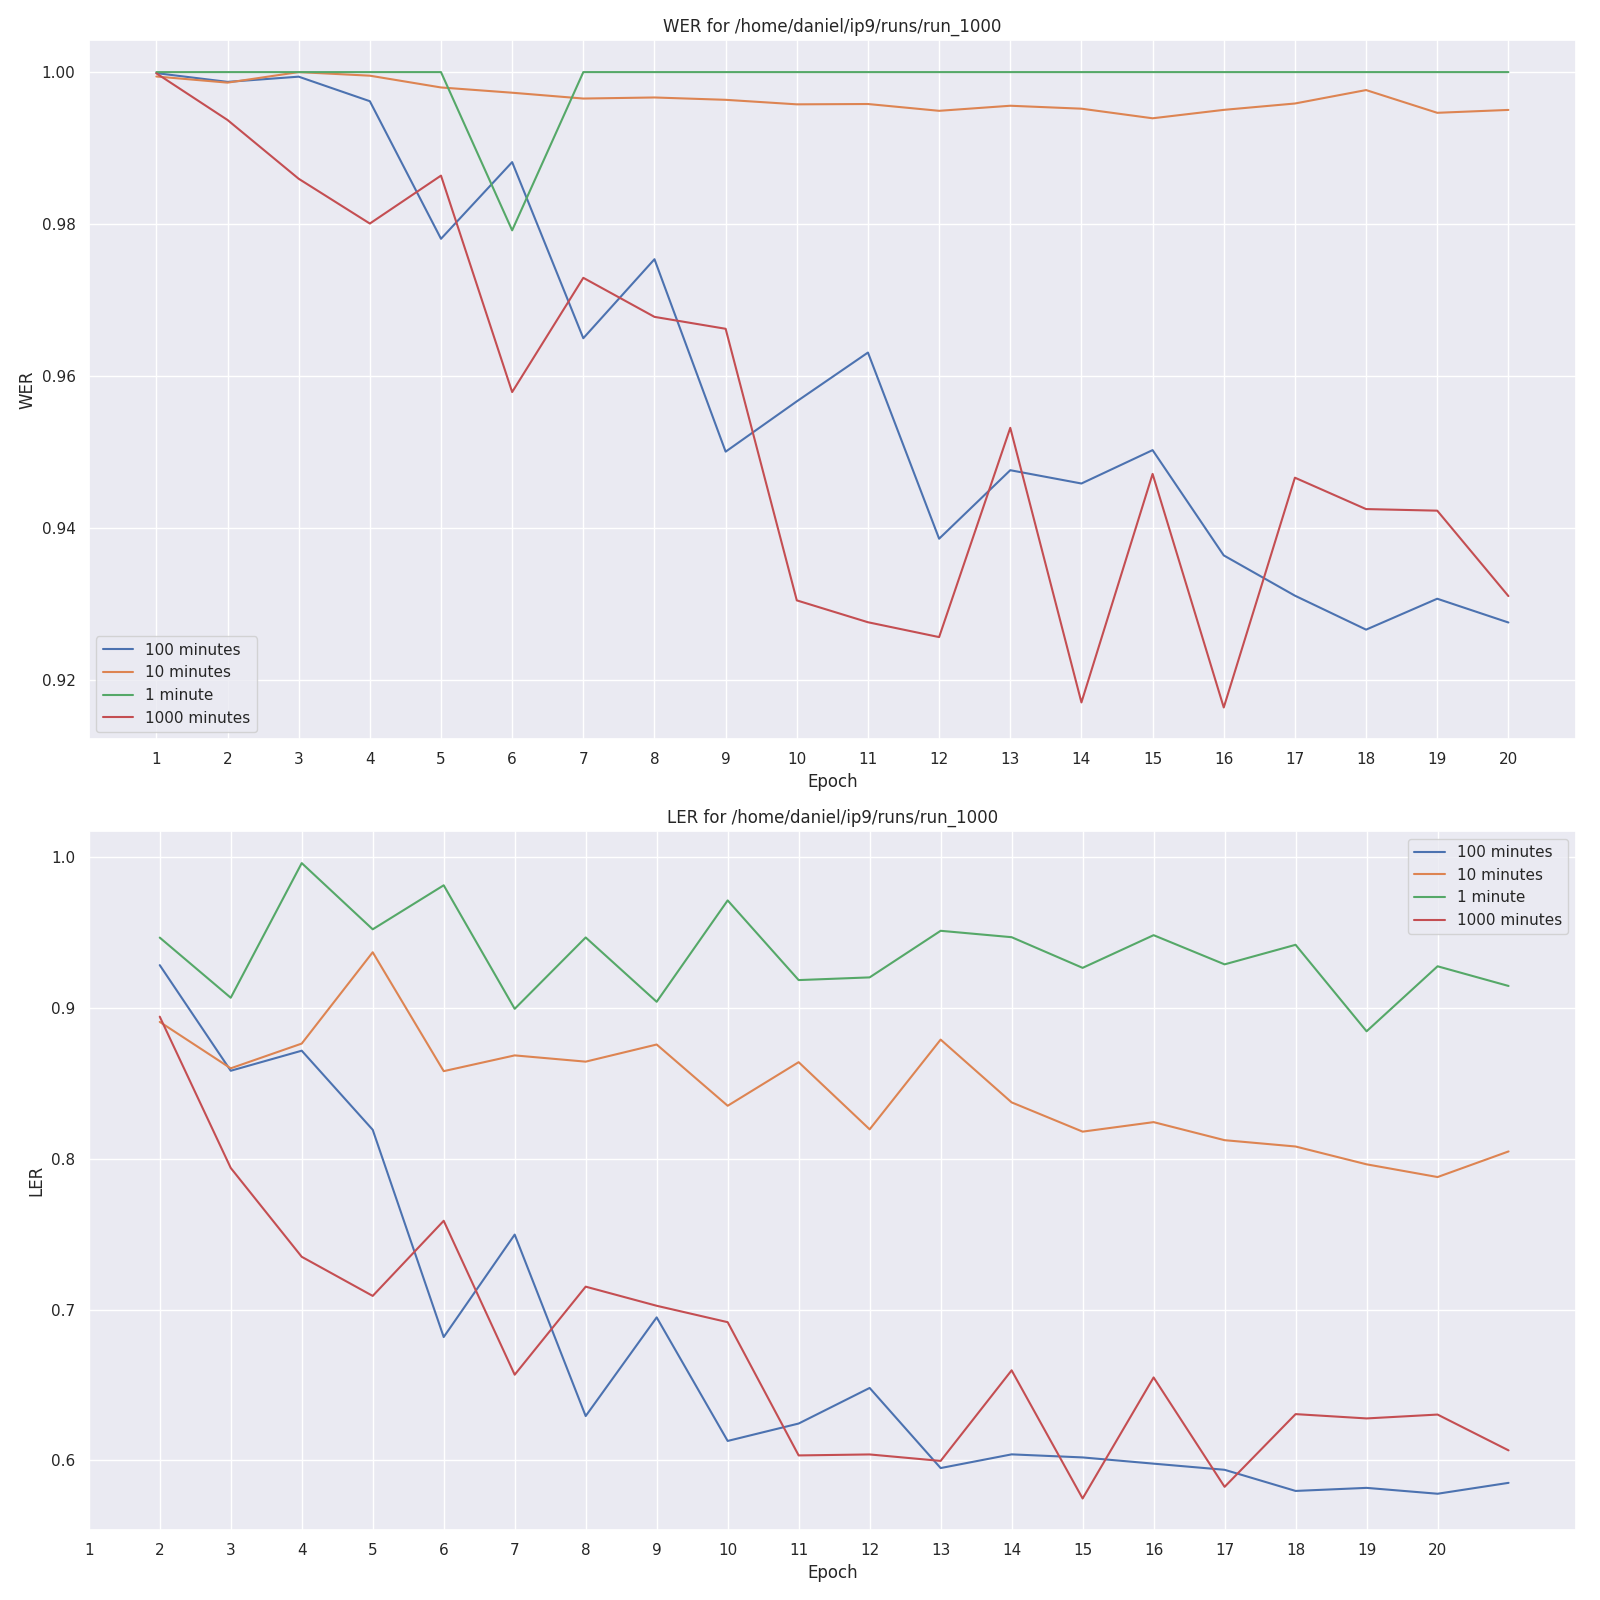
\includegraphics[width=\linewidth]{./img/learning_curve_lm_beamsearch.png}
	\caption{Learning curve for training on 1/10/100/1000 minutes of transcribed audio from \textit{ReadyLingua} using a 2-gram \ac{LM} and Beam-Search decoding}
\end{figure}

% To do:
% - train on LibriSpeech data
% - train using Best-Path
% - train using no LM
% - Reset calculation of WER/LER to original implementation
\newpage

\section{Creating a Language Model for German}\label{lm}

The learning curve above was plotted using the results from training on English samples. To compare get an intuition about whether the conclusions made are transferable to training on samples in other languages, the training was done again on German samples. In order to do this, a \ac{LM} for German had to be created first.

\subsection{n-Gram Language Models}

To understand the following sections better it might be helpful to get a quick recap about \ac{LM}. \ac{LM} are probabilistic models that model the likelyhood of a given sequence of characters or words. The most widely used type for word-based models \ac{LM}s are $n$-gram \ac{LM}. However, such models can estimate probabilities only for words that appear in the vocabulary of the corpus they were trained on. All other words are \ac{OOV} words with a probability of $0$. Single words are $1$-grams, but the same applies for $n$-grams of any order. But because of combinatorial explosion the $n$-gram, such \ac{LM} suffer from sparsity with increasing order $n$. To handle \ac{OOV} issues efficiently, a technique called \textit{smoothing} is applied. A very rudimentary form of smoothing is \textit{Laplace Smoothing}, which assigns a minimal count of $1$ to every $n$-gram. All other counts are also increased by adding $1$. This prevents counts of zero, which is important when calculating the perlexity of a model (because the count appears in the divisor and we cannot divide by zero) Although with Laplace Smoothing a very low probability is assigned to previously unseen $n$-grams (which results in a high perplexity), it performs poorly in application. A better way of smoothing is achieved using \textit{Kneser-Ney Smoothing}.

\subsection{Creating a raw text corpus and training the model}

A LM was trained on a raw text corpus of German Wikipedia articles using KenLM \parencite{kenlm}. The articles were pre-processed to meet the requirements of \textit{KenLM}.
It was normalized by removing Wiki markup, punctuation and making everything lowercase. Accentuated characters (like \code{è,é,ê}, etc.) and special characters like the German \textit{ß} were translated to their most similar ASCII-equivalent (\code{e} resp. \code{ss}) to account for ambiguous spelling and reduce the number of words. Umlauts (although not part of the ASCII codeset) were kept as-is because they are used very frequently in German.

Because \textit{KenLM} expects the input as sentences (one sentence per line), the raw text was further tokenized into sentences and words using NLTK \parencite{nltk}. Word tokens that contain only numeric characters (such as year numbers) are changed to \code{<unk>}, a special token which is traditionally used to denote an \ac{OOV} word. Although numeric tokens occur frequently in the Wikipedia articles, they are unwanted in the corpus because they do not carry any semantic meaning and because there is an infinite number of possible numbers.

The following lines are an excerpt of a article in the German Wikipedia along with its representation in the corpus.

\begin{displayquote}[German Wikipedia article about Speech Recognition\footnote{\url{https://de.wikipedia.org/wiki/Spracherkennung}}]
Die Größe des Wörterbuchs hängt stark von der Sprache ab. Zum einen haben durchschnittliche deutschsprachige Sprecher mit circa 4000 Wörtern einen deutlich größeren Wortschatz als englischsprachige mit rund 800 Wörtern. Außerdem ergeben sich durch die Flexion in der deutschen Sprache in etwa zehnmal so viele Wortformen, wie in der englischen Sprache, wo nur viermal so viele Wortformen entstehen.
\end{displayquote}

\begin{lstlisting}[numbers=left, caption=Representation in corpus]
die grösse des wörterbuchs hängt stark von der sprache ab
zum einen haben durchschnittliche deutschsprachige sprecher mit circa <unk> wörtern einen deutlich grösseren wortschatz als englischsprachige mit rund <unk> wörtern
ausserdem ergeben sich durch die flexion in der deutschen sprache in etwa zehnmal so viele wortformen wie in der englischen sprache wo nur viermal so viele wortformen entstehen
\end{lstlisting}

The final corpus contained data from 2,221,101 Wikipedia articles (42,229,452 sentences, 712,167,726 words, 8,341,157 unique words). A $4$-gram \textit{KenLM} model was trained on this corpus. KenLM uses \textit{Kneser-Ney Smoothing} and automatically adds the unigrams \code{<s>, </s>} and \code{<unk>} internally for sentence beginnings, endings and \ac{OOV} words). $n$-grams can be represented with a tree structure \footnote{note that \textit{KenLM} offers a so called \textit{PROBING} data structure, which is fundamentally a hash table combined with interpolation search, a more sophisticated variant of binary search, which allows for constant space complexity and linear time complexity. This does however not change the fact that $n$-grams can conceptually be thought as a tree of grams}, which allows for pruning. Pruning 1-grams would help getting rid of obvious spelling mistakes and very rare tokens that only appear in very special contexts. Unfortunately, \textit{KenLM} does not support pruning unigrams, only higher-order $n$-grams. Therefore the vocabulary used for training was limited to the 500,000 most frequent words not containing numbers with a minimum length of 2 characters \footnote{this constraint was imposed because NLTK did sometimes not tokenize abbreviations like \textit{z.B.} correctly, which resulting in two separate tokens \code{z} and \code{b}}. This amount is about the same what was used in the \textit{DeepSpeech} paper \parencite{deepspeech}. The words in the vocabulary make up 96.42\% of the whole corpus. The most frequent word in the vocabulary is the \code{<num>} token (29,659,021 counts), the least frequent word is \textit{Flachmeeres} (31 counts). Note that the latter is actually a derivate of another German word \textit{Flachmeer}, which also appears in the vocabulary (109 counts). Having different flexions of the same word is characteristic for German texts. Handling them would require lemmatization and/or stemming the corpus, which has not been done for simplicity. It is also doubtful whether this would actually help improving the quality of inferred transcripts, since humans do not speak in lemmata or stems.

By limiting the vocabulary to the 500k most frequent words, the unigrams in the KenLM were artificially pruned. The number of unigrams was therefore 500,003 (one unigram for each word in the vocabulary plus one each for the \code{<s>}, \code{</s>} and \code{<unk>} tokens). The $n$-grams used to train the \ac{LM} have been pruned by setting the minimal threshold for $n$-Grams of any order ($n \in 1..4$) to 40. This is the value that Google used (reference from Jurafsky). Pruning unigrams helped getting rid of obvious spelling mistakes and very rare tokens that only appear in very special contexts (like the tokens \textit{aaaaa} or \textit{zzyzzyxx}) (EDIT: Pruning unigrams is not supported by KenLM, but the vocabulary can be limited). Such words are mostly not no real German words and should therefore not be trained on. Pruning higher-order $n$-grams was done to increase performance (both in space and time).

\subsection{Evaluating the model}

The best way to evaluate a \ac{LM}is to embed it in an application and measure how much the application improves \parencite{slp3}. This is called \textit{extrinsic evaluation} and has been done by comparing the learning curves with and without using a \ac{LM}. However, to measure the performance of a \ac{LM} independently (\textit{intrinsic evaluation}) one would have to provide a test set containing unseen sentences an assess the scores of the \ac{LM} on their $n$-grams. The results can then be compared to a reference \ac{LM}: Whatever model produces higher probabilities (or lower perplexity) to the $n$-grams in the test set is deemed to perform better. However, because models can only be compared if they use the same vocabulary \parencite{slp3}, this would require training the reference model would need to be trained on the same corpus, which can become very time consuming.

\textit{KenLM} has been extensively compared to other \ac{LM} implementations like \ac{SRILM} both in terms of speed and accuracy. It has been found to be both faster and more memory efficient \parencite{kenlm} than the fastest alternative. Its low memory profile makes it runnable on a single machine, while other algorithms like \textit{MapReduce} target clusters \parencite{kenlm_estimation}. This was a big advantage especially for this project. The probabilistic performance of \textit{KenLM} has been evaluated by training a $5$-gram model on a 126 billion token corpus (393 unique words) \parencite{kenlm_estimation}. This model was embedded in some Machine Translation systems (Czech-English, French-English and Spanish-English) . Evaluation was done by calculating the BLEU score and comparing it to embeddings of other \ac{LM}. \textit{KenLM} placed first in all submissions.

Because of time constraints and because \textit{KenLM} has already been extensively evaluated on English I resign from evaluating my German \ac{LM} intrinsically, although the corpus used for training is not as big as the one used in \cite{kenlm_estimation}. To this day \textit{KenLM} is widely recognized as the best performing \ac{LM} out there, which is also emphasized by the usage of a \textit{KenLM} model in the Mozilla implementation of \textit{DeepSpeech}.

To still get an intuition about how well the model performs, two different experiments were made:

\begin{itemize}
	\item \textbf{Experiment 1}: The probability calculated for valid German sentences was compared against variants of the same sentences where the words appear in randomized order.
	\item \textbf{Experiment 2}: The \ac{LM} was used together with its vocabulary to build a simple word predictor.
\end{itemize}

Both experiments are explained in more depth below.

\subsubsection{Evaluation 1: Comparing scores of randomized sentences}

The first experiment tests the validity of the probabilities (\textit{scores}) calculated by the \ac{LM}. For this, an arbitrary choice of 5 valid sentences in German was used. To make sure the sentences could not have been seen during training, the following 5 sentences were taken out of the current newspaper (dated after the creation of the Wikipedia dump):

\begin{itemize}
	\item \textit{Seine Pressebeauftragte ist ratlos.}
	\item \textit{Fünf Minuten später steht er im Eingang des Kulturcafés an der Zürcher Europaallee.}
	\item \textit{Den Leuten wird bewusst, dass das System des Neoliberalismus nicht länger tragfähig ist.}
	\item \textit{Doch daneben gibt es die beeindruckende Zahl von 30'000 Bienenarten, die man unter dem Begriff «Wildbienen» zusammenfasst.}
	\item \textit{Bereits 1964 plante die US-Airline Pan American touristische Weltraumflüge für das Jahr 2000.}
\end{itemize}

For each of these sentences the score was calculated. Then the words of the sentences were shuffled and the score was calculated again. A good \ac{LM} should calculate a (much) higher probability for the original sentence, because the shuffled sentence is most likely to be gibberish. All sentences have been normalized the same way sentences were preprocessed for training. Table \ref{LM_evaluation} shows the results of the comparison. It is evident that the probabilities for the shuffled sentences are much lower than for the sentences where the words appear in the correct order. The probabilities calculated by the \ac{LM} are therefore deemed valid.

\begin{table}[!htbp]
	\centering
	\begin{tabular}{|l|r|l|r|}
		\hline
		\thead{original sentence (normalized)} & \thead{score} & \thead{permuation} & \thead{score} \\
		\hline
		\makecell[l]{seine pressebeauftragte\\ist ratlos} & -17.58 & \makecell[l]{ist ratlos\\pressebeauftragte seine} & -21.52 \\
		\hline
		\makecell[l]{fünf minuten später steht\\er im eingang des kulturcafes\\an der zürcher europaallee} & -40.23 & \makecell[l]{des er minuten zürcher kulturcafes\\steht europaallee eingang\\fünf im später an der} & -57.69 \\
		\hline
		\makecell[l]{den leuten wird bewusst\\dass das system des \\ neoliberalismus nicht\\länger tragfähig ist} & -35.52 & \makecell[l]{system nicht das ist\\dass leuten tragfähig des\\neoliberalismus den\\bewusst länger wird} & -51.27 \\
		\hline
		\makecell[l]{doch daneben gibt es die\\beeindruckende zahl von \code{<num>}\\bienenarten die man unter dem\\begriff wildbienen zusammenfasst} & -48.36 & \makecell[l]{dem gibt wildbienen zahl\\beeindruckende doch man\\zusammenfasst es daneben bienenarten\\von die unter die \code{<num>} begriff} & -75.95 \\
		\hline
		\makecell[l]{bereits \code{<num>} plante\\die usairline pan american\\touristische weltraumflüge\\für das jahr \code{<num>}} & -58.04 & \makecell[l]{plante touristische für\\jahr pan american das\\bereits usairline \code{<num>}\\\code{<num>} weltraumflüge die} & -64.02 \\
		\hline
	\end{tabular}
	\caption{Comparison of log10-probabilities calculated for news sentences and a permutation of their words}
	\label{LM_evaluation}
\end{table}

\subsubsection{Experiment 2: Word predictor}

The second experiment tests whether the trained \ac{LM} is able to continue a sentence given its beginning. For this each word from the vocabulary is appended and the score of the resulting stumps is calculated. The most likely continuation can be estimated by sorting the resulting list in descending order (the probabilities are $\log_10$-based, i.e. negative) and taking the first element. This behavior can be applied iteratively to construct a sentence from a stump. For this experiment a sentence was started with the stump \textit{Ein - 2007 - erschienenes}. Afterwards a word from the five most probable continuations was appended. The extended stump was then again fed into the \ac{LM}. This process was repeated until some kind of sentence ending was encountered. Eacg extended stump was preprocessed the same way the sentences were preprocessed for training (lowercasing, replacing numbers with \code{<num>}, etc.). Figure \ref{word_predictor} shows the path taken through the predictions. Note that the predictions for the second and third word of the stump after typing the first word are shown in grey for illustrative purposes, although they were not considered for continuation.

\begin{figure}
	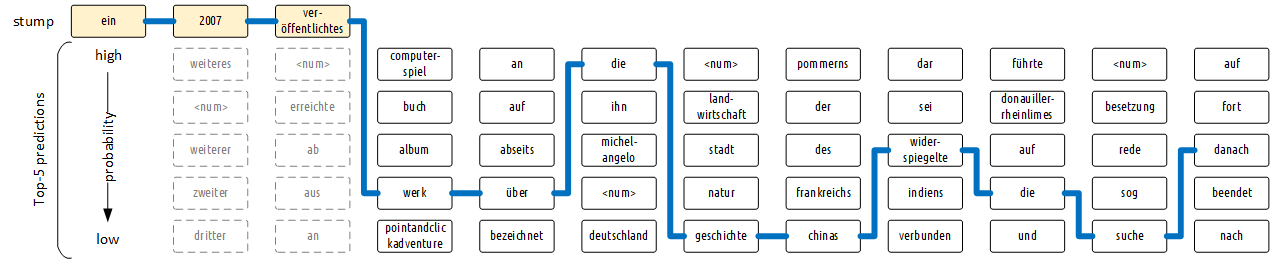
\includegraphics[width=\linewidth]{./img/word_predictor.png}
	\caption{Word predictions of the trained 5-gram model for continuations of the stump \textit{«Ein 2007 erschienenes ...»}. The blue path represents a grammatically valid German sentence.}
	\label{word_predictor}
\end{figure}

Although prediction was slow we can observe that the words suggested by the \ac{LM} are generally grammatically correct continuations and often make sense, although the probability for some of the predicted words (like \textit{Michelangelo}) is sometimes unexplicably high. Nevertheless it was possible to create a grammatically correct German sentence from the stump using only the suggested words. The \ac{LM} even seems to have captured some notion about grammatical concepts like German cases (e.g. that \textit{"die Geschichte Chinas"} is more likely than \textit{"die Geschichte China"}). On the other hand we can observe that the meaningfulness of the suggestions decreases with the progress because some long-distance relationships between words are lost for small values of $n$.

%score for 'ein': -2.5511488914489746
%top 5 words:
%word        log10-probability
%--------  -------------------
%weiteres             -5.973
%<num>                -6.00614
%weiterer             -6.18446
%zweiter              -6.21412
%dritter              -6.30031
%
%score for 'ein <num>': -4.864611625671387
%top 5 words:
%word         log10-probability
%---------  -------------------
%<num>                 -7.34603
%erreichte             -7.75604
%ab                    -7.77345
%aus                   -7.86214
%an                    -7.87674
%
%score for 'ein <num> erschienenes': -7.372537136077881
%top 5 words:
%word                      log10-probability
%----------------------  -------------------
%computerspiel                      -8.47756
%buch                               -8.86841
%album                              -9.2071
%werk                               -9.30259
%pointandclickadventure             -9.31129
%
%score for 'ein <num> erschienenes werk': -8.43615436553955
%top 5 words:
%word          log10-probability
%----------  -------------------
%an                     -10.5713
%auf                    -10.863
%abseits                -10.9379
%über                   -11.0053
%bezeichnet             -11.0132
%
%score for 'ein <num> erschienenes werk über': -9.723254203796387
%top 5 words:
%word            log10-probability
%------------  -------------------
%die                      -12.0887
%ihn                      -12.1763
%michelangelo             -12.4766
%<num>                    -12.4973
%deutschland              -12.5661
%
%score for 'ein <num> erschienenes werk über die': -9.965542793273926
%top 5 words:
%word              log10-probability
%--------------  -------------------
%<num>                      -11.9341
%landwirtschaft             -12.1469
%stadt                      -12.2681
%natur                      -12.2898
%geschichte                 -12.5322
%
%score for 'ein <num> erschienenes werk über die geschichte': -11.084966659545898
%top 5 words:
%word           log10-probability
%-----------  -------------------
%pommerns                -12.7682
%der                     -13.4756
%des                     -13.5903
%frankreichs             -13.6889
%chinas                  -13.7065
%
%score for 'ein <num> erschienenes werk über die geschichte chinas': -13.830591201782227
%top 5 words:
%word              log10-probability
%--------------  -------------------
%dar                        -14.8973
%sei                        -14.9483
%widerspiegelte             -15.1113
%indiens                    -15.555
%verbunden                  -15.6136
%
%score for 'ein <num> erschienenes werk über die geschichte chinas widerspiegelte': -15.959598541259766
%top 5 words:
%word                    log10-probability
%--------------------  -------------------
%führte                           -19.0873
%donauillerrheinlimes             -19.3014
%auf                              -19.3185
%die                              -19.3199
%und                              -19.3243
%
%score for 'ein <num> erschienenes werk über die geschichte chinas widerspiegelte die': -17.793916702270508
%top 5 words:
%word         log10-probability
%---------  -------------------
%<num>                 -19.5746
%besetzung             -20.353
%rede                  -20.706
%sog                   -20.7197
%suche                 -20.7211
%
%score for 'ein <num> erschienenes werk über die geschichte chinas widerspiegelte die suche': -19.95460319519043
%top 5 words:
%word       log10-probability
%-------  -------------------
%auf                 -21.5493
%fort                -21.8571
%danach              -21.8975
%beendet             -22.052
%nach                -22.0672

%score for 'ein <num> erschienenes werk über die geschichte chinas widerspiegelte die suche danach': -22.0571231842041
%top 5 words:
%word           log10-probability
%-----------  -------------------
%diskutiert              -23.6575
%abzielen                -23.9694
%begeben                 -23.9833
%beeinflusst             -24.0387
%auf                     -24.0435
\newpage

\section{Learning curve}

This section describes how training progress was estimated by plotting a learning curve.

\subsection{Previous corpora and their problems}

The following two corpora were available for training from the IP8 project.

\begin{itemize}
	\item \textbf{\ac{LS}}: This corpus was created as an artifact of the IP8 project using raw data from OpenSLR. The raw is publicly available and can be downloaded\footnote{\url{http://www.openslr.org/12/}}. It consists of a number of audio files which were \textit{partially} transcribed, i.e. there are parts in the audio for which the corresponding transcript is not exactly known (the audio contains \textit{gaps}). The individual samples were obtained by exploiting metadata included in the download. The metadata includes a split into a training set (containing approximately 96\% of the samples) and a validation resp. test set (each containing approximately 3\% of the samples). The split was done manually into disjoint subset, i.e. ensuring each speaker was only included in one set. Additionally, other features like gender or accent were observed to achieve a similar distribution for each set. To leverage the efforts made by \textit{OpenSLR}, this split was not changed.
	\item \textbf{\ac{RL}}: This corpus was created from raw data provided by \textit{ReadyLingua}. This data is proprietary and contains recordings in several languages which were manually aligned with their transcript. In contrast to the \ac{LS} corpus, the raw data is fully aligned, i.e. there are no gaps in the audio. However, the metadata does not comprise a split into training-, validation- and test-set. Since the raw data contained recordings and transcripts in more than one language, separate splits were made for each language preserving a ratio of approximately 80/10/10\% (relating to the total length of all recordings within each subset). Efforts were made to prevent samples from the same recording being assigned to different subsets. Other features were not observed, meaning the split into train/validation/test-set was done less carefully than in the \ac{LS} corpus.
\end{itemize}

The model in the IP8 project was supposed to be trained on the \ac{LS} corpus, because this corpus is much larger than the \ac{RL} corpus. In the course of the project it became clear however that training on all samples from this corpus was not feasible within project time because training time would have taken more than two months. It also turned out that the \ac{LS} corpus was probably less useful than initially assumed because the average sample length was much longer than the samples in the \ac{RL} corpus. This made training even harder because convergence is much slower when training on long sequences. The \ac{RL} corpus on the other hand consisted of shorter samples, but the total length of all samples was only a few hours compared to the 1000+ hours in the \ac{LS} corpus.

\subsection{The \textit{CommonVoice} (\ac{CV}) Corpus}

Because of the aforementioned problems a new corpus was needed which combined the best of both worlds:

\begin{itemize}
	\item it should contain a reasonable amount of speech samples to facilitate training an ASR model
	\item the average sample length should be short enough for the model to learn quickly.
\end{itemize}

The \ac{CV}\footnote{\url{https://voice.mozilla.org/en/data}} corpus is built and maintained and used actively by the Mozilla Foundation and exhibits both of these properties. This corpus is also used to train the Mozilla implementation of \textit{DeepSpeech}. Datasets for various languages are being prepared and verified, each one containing speech samples of different contributors from all over the world. At the time of this writing, only the English dataset was available, but datasets for other languages will become publicly available at some time in the future. The English dataset comes pre-divided into training-, validation- and test-set of similar scale like the \ac{LS} corpus. Each set consists of one audio file per sample and a CSV file containing the transcriptions for each sample.

For this project the English dataset was used to train the simplified model. Although still smaller than than the \ac{LS} corpus, the total length of all validated samples that can be used for training\footnote{CSV file: \code{cv-valid-train.csv}} is much larger than the \ac{RL} corpus while providing samples of similar length at the same time. Table \ref{corpora_stats} shows some statistics about the corpora described above.

\begin{table}[!htbp]
	\centering
	\begin{tabular}{|l|l|r|r|r|r|r|}
		\hline
		\thead{Corpus} & \thead{Language} & \thead{total audio length} & train/dev/test & \thead{\# samples} & \thead{Ø sample length} & \thead{Ø transcript length} \\
		\hline
 		\ac{LS} & English & $24 days, 7:13:18$ & $93.51/3.32/3.16\%$ & $166,510$ & $12.60$ & $183.84$ \\ 
		\ac{RL} & English & $5:38:39$ & $80.39/10.13/9.48\%$ & $6,334$ & $3.20$ & $51.81$ \\ 		
		\ac{RL} & German & $1:58:30$ & $81.14/10.26/8.60\%$ & $2,397$ & $2.89$ & $45.55$ \\ 		
		\ac{CV} & English & $10 days, 1:02:53$ & $96.04/1.99/1.98\%$ & $201,252$ & $4.31$ & $48.07$ \\ 
		\hline
	\end{tabular}
	\caption{Statistics about corpora that were available for training. The sample lenght is given in seconds, the transcript length as the number of characters.}
	\label{corpora_stats}
\end{table}

\subsection{Plotting the learning curve}

The time needed to train an \ac{ASR} model on all samples of the \ac{CV} corpus is still too long for the available project time. We can however still get an estimate of the learning progress by plotting a \textit{learning curve}. For this, exponentially increasing amounts of training data (1, 10, 100 and 1,000 minutes of transcribed audio) were used. Training was done making 30 full passes (\textit{epochs}) over the training data. After each epoch, the progress was monitored by inferring the transcriptions for previously unseen samples from the validation set. The \ac{CTC}-loss for training and validation was plotted for each amount, yielding separate curves for the training- and the validation-loss. Comparing both curves allows for making statements about at what point the Neural Network starts to overfit.

Complementary to the \ac{CTC}-loss, the mean values for the \ac{LER} and \ac{WER} metric over all samples in the validation set is calculated after each epoch, yielding the curves for the \ac{LER} resp. \ac{WER}. Observing these plots can give some insight about how well the network performs on unseen examples.

Both loss and metrics were compared along two dimensions:

\begin{itemize}
	\item \textbf{The decoder dimension}, comparing the two distinct ways to decode a transcript from the probability distributions calculated by the model for each frame in the input signal
	\item \textbf{The LM dimension}, comparing inferences made with and without post-processing the decoded transcript with a spell-checker as described above
\end{itemize}

Both dimensions are described in more detail below.

\subsubsection{Decoder dimension}

In a nutshell, \ac{CTC} aligns the $T_y$ characters from a known transcription (\textit{label}) with the $T_x$ frames from the input audio signal during training. $T_x$ is typically much larger than $T_y$ and must not be shorter. The characters (\textit{tokens}) in the label must come from an alphabet of size $V$, which for English are the 26 lowercased ASCII characters $a..z$, the space character and the apostrophe (because this character is very common in abbreviations like e.g. \textit{"don't"} or \textit{"isn't"}). Additionally, \ac{CTC} introduces a special token $\epsilon$, called the \textit{blank token}, which can be used to label unknown/silent frames or prevent collapsing (see below). Consequently, the number of characters in the alphabet used by the \ac{ASR} in this project to recognize English is $V=26+1+1+1=29$.

\ac{CTC} is \textit{alignment-free}, i.e. it does not require an alignment between the characters of a transcription and the frames of an audio signal. The only thing needed is the audio signal $X$ itself plus its ground truth $Y$. Each token in the ground truth can be aligned with any number of frames in the input signal. Vice versa, repeated sequences of the same characters can be collapsed, whereas the $\epsilon$ token functions acts as a boundary within sequences of a token to prevent collapsing into one, when there should be two (such as in \textit{g-g-o-o-$\epsilon$-o-o-o-o-d-d-d}, which should collapse to \textit{good} and not \textit{god}). 

For each frame input signal \ac{CTC} calculates a probability distribution over th $V$ characters in the alphabet. This yields a $V \times T_x$ probability matrix for the input signal. Because $T_x >> T_y$, there is usually a vast amount of different valid alignments collapsing to the ground truth. The probability of each valid alignment can now simply be calculated by traversing the probability matrix from left to right and multiplying the probabilities of each character. Because calculating the probability of each valid alignment individually would be too slow and identical prefixes between valid alignments yield identical probabilities, a dynamic approach is usually chosen to calculate the probabilities whereas the intermediate probability for each prefix is saved once computed.

The most probable alignment is calculated by marginalizing (i.e. summing up) over the probabilities of the individual valid alignments. This calculation yields the CTC loss as a sum of products, which is differentiable and can therefore be optimized.

After training, a model using \ac{CTC} will again output a $V \times T_x$ probability matrix for any previously unseen input. This matrix can be used to infer a transcription, a process also known as \textit{decoding}. The \ac{CTC} paper proposes two different decoding strategies that are applied before collapsing the characters \cite{ctc_paper}:

\begin{itemize}
	\item \textbf{Best-Path (a.k.a. \textit{greedy}) decoding}: This strategy only ever considers the most likely character at each time step. The transcription before collapsing will be a single path through the the probability matrix, whose probability will be the product of all elements along the path. This approach is easy to implement but does not take into account the fact that a single output can have many alignments, whose individual probability may be lower than the one found with this strategy.
	\item \textbf{Beam-Search decoding}: This strategy approximates the probability of the most probable transcription by following multiple paths simultaneously and only keeping the $B$ most probable paths at each time step. The beam width is a hyperparameter that can be increased to get a more accurate transcription in exchange for higher computational cost.
\end{itemize}

Usually, Beam-Search decoding performs better than Best-Path decoding. For the sake of completeness, both decoding strategies were compared in this project. This will yield separate learning curves for the decoder dimension. For Beam-Search decoding, the Keras implementation was used, which proposes a default beam width of $B=100$. This value was not changed. 

\subsubsection{\ac{LM} dimension}

Using a \ac{LM} to post-process the inferred transcription with a rudimentary spell checker will not necessarily lead to more accurate transcription, especially if the edit distance between prediction and ground truth is large. Figure \ref{lm_dimension_example} contains some examples where the use of a spell checker is disadvantageous to the quality of a transcription.

\begin{figure}[h!]
	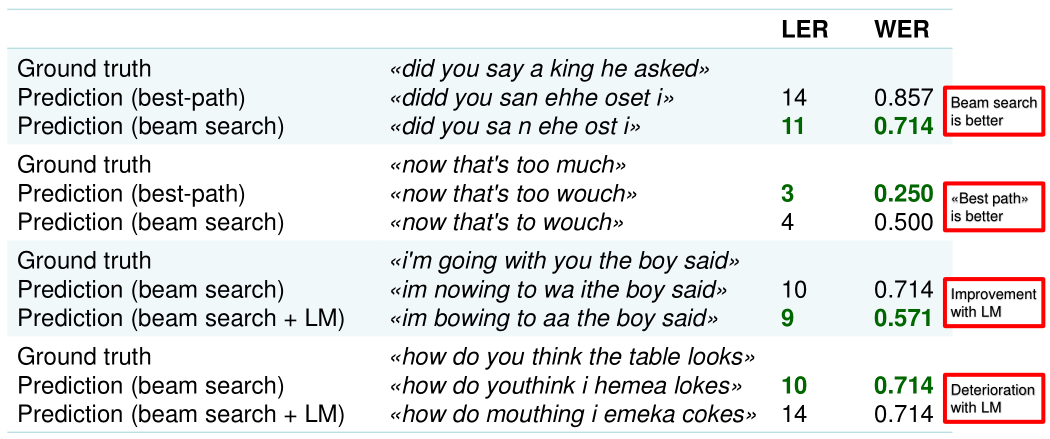
\includegraphics[width=\linewidth]{./img/lm_dimension_example.png}
	\caption{Example of how a spell checker can improve or deteriorate the quality of a prediction.}
	\label{lm_dimension_example}
\end{figure}

In this example, \textit{"how do youthink i hemea lokes"} was changed to \textit{"how do mouthing i emeka cokes"} because \textit{youthink}was not in the vocabulary and \textit{mouthing} was the most probable word with a maximum edit distance of 2 that was in the vocabulary. Similarly, \textit{lokes} was changed to \textit{cokes}. This lead to a orthographically better sentence, but the \ac{LER} is higher than without spell-checking. 

It is generally expected that post-processing the inference as described above will lead to a lower \ac{WER}, supposed the \ac{LER} is already low enough, i.e. the prediction matches the ground truth already pretty well. If the \ac{LER} value is too high, the spell checker might try too hard to find a word from the vocabulary. This might result in a changed sentence consisting of real words but whose similarity to the ground truth is lower than before the changes. Post-processing might then be counter-productive. Therefore, separate learning curves were plotted for inference with and without post-processing (the \textit{\ac{LM} dimension})

\subsection{Results and interpretation}

Figure \ref{lc_loss_cv} shows the learning curve for the \ac{CTC}-loss. Obviously the training losses decrease steadily, converging to values between 30 (when training on 1.000 minutes) and 50 (when training on 1 minute). The validation losses (dashed lines) start to increase after 10 to 15 epochs, although the trend is less evident for smaller amounts of training data because the curves are oscillate and are somewhat less smooth. This means the network will start to overfit after 10 to 15 epochs and generalize worse with each additional training epoch.

Figure \ref{lc_ler_cv} shows the progress of the \ac{LER} with and without spelling correction for each of the decoder dimensions. Figure \ref{lc_wer_cv} does the same for the \ac{WER}. It is evident that the \ac{LER} will converge to a minimum value of about 0.54 when using best-path decoding and 0.52 when using beam search. Post-processing the transcript using a spell-checker does not seem to have great impact. In fact it will even produce slightly higher \ac{LER} values for beam search decoding. This behavior is expected considering the observations described for the \ac{LM} dimension above.

\begin{figure}[h!]
	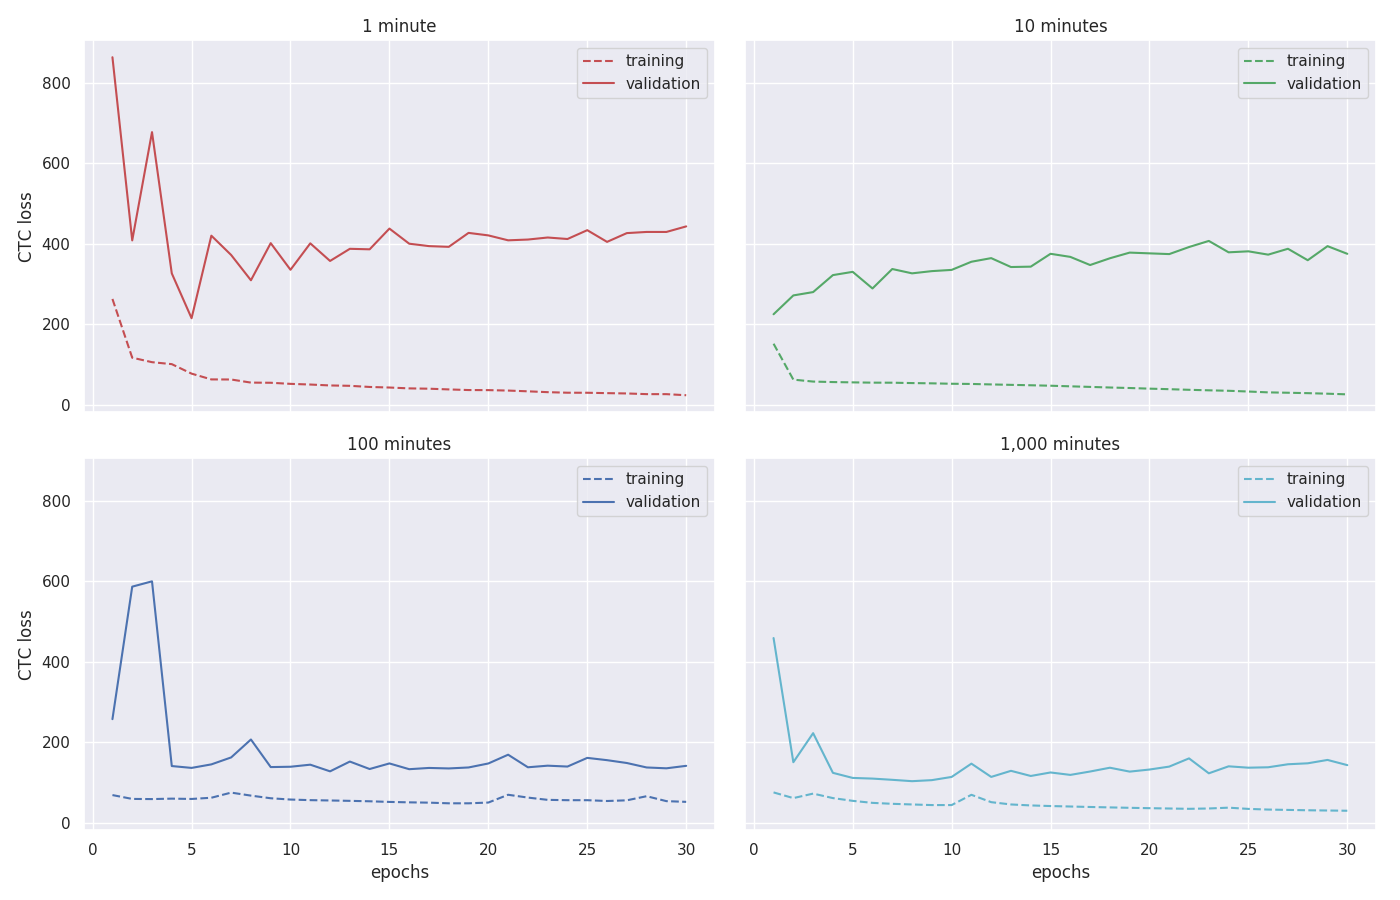
\includegraphics[width=\linewidth]{./img/lc_loss_cv.png}
	\caption{Learning curve for the CTC-loss while training on 1/10/100/1000 minutes of transcribed audio from the \ac{CV} corpus using the $5$-gram \ac{LM} provided by the Mozilla implementation of \textit{DeepSpeech}}
	\label{lc_loss_cv}
\end{figure}

\begin{figure}[h!]
	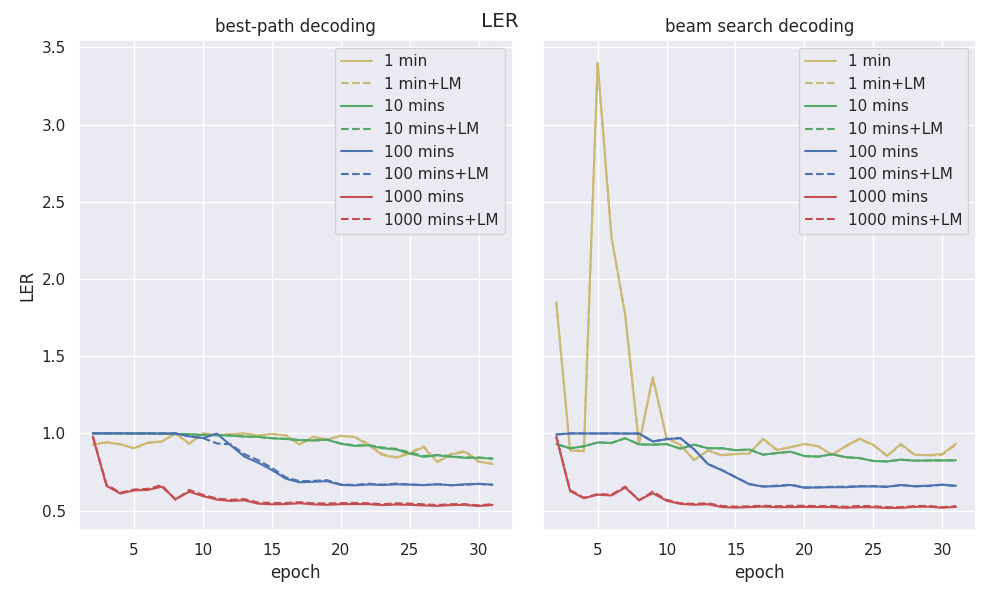
\includegraphics[width=\linewidth]{./img/lc_ler_cv.png}
	\caption{Learning curve for the \ac{LER} metric while training on 1/10/100/1000 minutes of transcribed audio from the \ac{CV} corpus with and without spelling correction with a \ac{LM}. For the lines where spelling was corrected, the $5$-gram \ac{LM} provided by the Mozilla implementation of \textit{DeepSpeech} was used.}
	\label{lc_ler_cv}
\end{figure}

\begin{figure}[h!]
	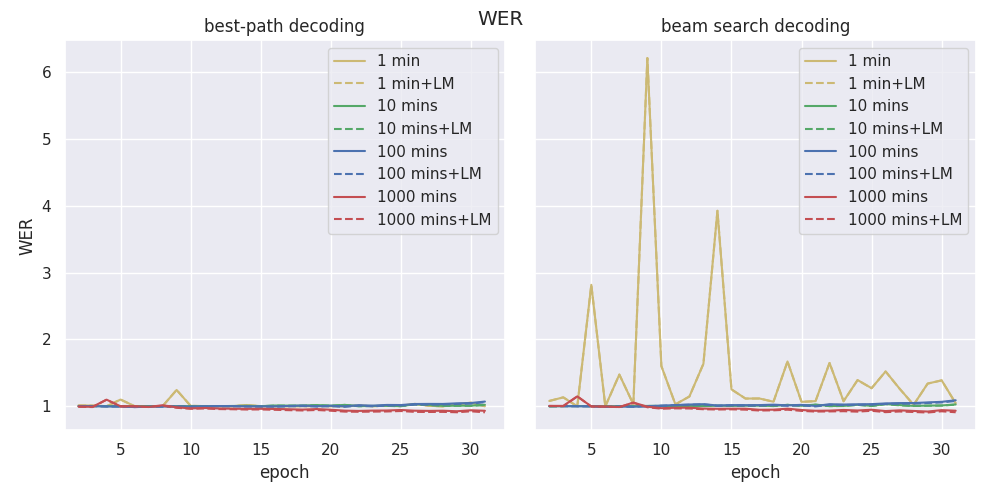
\includegraphics[width=\linewidth]{./img/lc_wer_cv.png}
	\caption{Learning curve for the \ac{WER} metric while training on 1/10/100/1000 minutes of transcribed audio from the \ac{CV} corpus with and without spelling correction with a \ac{LM}. For the lines where spelling was corrected, the $5$-gram \ac{LM} provided by the Mozilla implementation of \textit{DeepSpeech} was used.}
	\label{lc_wer_cv}
\end{figure}

\subsection{Regularization}


\subsection{Final thoughts and considerations}

Above results were achieved using the 5-gram \ac{LM} from Mozilla 

Reversing 

%Hier etwas über
%
%- Batchgrösse (Qualität nimmt mit zunehmender batchgrösse ab!)
%- Padding der Trainingssequenzen
%- Sortierung der Trainingsdaten nach Länge (ist besser, da weniger blanks gepadded, schnellere Konversion)
%- ...
%
%Beispiel für Prediction, wo LER/WER durch LM verschlechtert wurde: (aus /home/daniel/_runs/lc_bestpath_rlen/1000_min_bestpath/test_results.csv)
%
%#: 546	
%ground truth: i want to wish you a very happy thanksgiving	
%prediction: oento wiceyouepery appy thangksive (LER=0.431818181818182, WER=1)
%prediction (LM-corrected): onto wiceyouepery app thangksive	(LER=0.454545454545455	WER=1)
%
%
%
% To do:
% - train on LibriSpeech data
% - train using Best-Path
% - train using no LM
% - Reset calculation of WER/LER to original implementation


\newpage

\section{Measuring the performance of the pipeline}\label{e2e}

Above results reflect the performance of the \ac{ASR} model alone. To get some insight about the quality of alignments produced by the whole pipeline, a simple web application was implemented that highlights the aligned parts of the transcript as the audio file is being played. This is very useful for an informal review, because the subjective quality of the alignments can be examined interactively. However, this method is not very systematic and infeasible for larger amounts of test data. To get a clearer sense of how well the pipeline performed, steps were taken to run large numbers of previously unseen samples through the pipeline and measure the quality of the alignments produced. This section describes how this was done.

\subsection{The quality of alignments}

Assessing the quality of alignments is not trivial because there is often no reference alignment to compare to. Even if there is one, assessing the quality of an alignment is somewhat subjective because there is a a massive number of theoretically possible alignments for each transcript. We can however derive a few objective criteria that make up a good alignment:

\begin{enumerate}
	\item The aligned partial transcripts should not overlap each other
	\item The alignments should neither start nor end within word boundaries
	\item The aligned partial transcripts should cover the as much of the original transcript as possible	
	\item The aligned partial transcripts should be at the correct position (i.e. they should cover the actually spoken text)
\end{enumerate}

The first criterion is enforced by changing the type of algorithm used for sequence alignment from a local to a global alignment algorithm. During the IP8 project, the \textit{Smith-Waterman} algorithm was used in the \ac{LSA} stage, which finds a local optimum for each transcript individually. This was replaced by the \textit{Needle-Wunsch} algorithm, which finds an optimal alignment for all partial transcrips at once. 

The second criterion is ensured by adjusting some of the alignments produced by \textit{Needle-Wunsch} so that they fall exactly on word boundaries.

The remaining two criteria can be quantified with the following metrics (note the corellation\footnote{positive correlation: higher is better, negative correlation: lower is better}):

\begin{table}[!htbp]
	\centering
	\begin{tabular}{|l|l|l|l|}
		\hline
		\thead{criterion} & \thead{metric} & \thead{symbol} & \thead{correlation} \\
		\hline
		1 & \makecell[l]{length of text in ground truth that is not aligned vs. total length of the ground truth} & $C$ & negative \\ 
		\hline		
		3 & \makecell[l]{average Levensthein similarity between the transcript\\and the text in the ground truth corresponding to its alignment} & $D$ & positive \\ 
		\hline				
	\end{tabular}
	\caption{Metrics to evaluate the quality of alignments}
	\label{LM_evaluation}
\end{table}

Because the first metric measures how much of the target transcript is covered by the alignments, it is somewhat similar to the Recall $R$. The second metric measures how well the produced results match up with the underlying parts of the transcript and is therefore similar to Precision $P$. Both metrics can therefore be reduced to the F-score, a single number usually used to evaluate classification results:

\[ 
F = 2\cdot \frac{P\cdot R}{P+R}
 \]

Figure \ref{example_alignment} shows an example of an alignment. The sentence was split into speech segments by \ac{VAD} which were then aligned with the whole sentence (ground truth). Some speech segments were misaligned, resulting in an overlap. Some of the transcriptions contain mistakes. Note that the Levensthein Similarity ($ls(s_1, s_2)$) measures the similarity of two strings $s_1$ and $s_2$ as the normalized edit distance and is calculated as follows:

\begin{equation}
	ls(s_1, s_2) = 1 - \frac{ed(s_1, s_2)}{max \left(len(s_1), len(s_2), len(s_3)\right)}
\end{equation}

For $t_1=\text{i see}, t_2=\text{i c}, t_3 = \text{sad the blind men}, t_4 = \text{to his blind daughter}$ The metrics can be calculated as follows:

\begin{equation}
C = \frac{len(\text{i see})}{len(\text{i see i see said the blind man to his deaf daughter})} = \frac{5}{51} = 0.098
\end{equation}

\begin{equation}
\begin{split}
O & = \frac{len(\text{i see})}{len(\text{i see}) + len(\text{i c}) + len(\text{sad the blind men}) + len(\text{to his deaf daughter})} \\
 & = \frac{5}{5 + 3 + 17 + 20} = 0.11
\end{split}
\end{equation}

\begin{equation}
\begin{split}
D & = \frac{ls(\text{i see}, t_1) + ls(\text{i see}, t_2) + ls(\text{said the blind man}, t_3) + ls(\text{to his deaf daughter}, t_4)}{4} \\
 & = \frac{1 + 0.4 + 0.88 + 1}{4} = 0.82
\end{split}
\end{equation}

\begin{figure}
	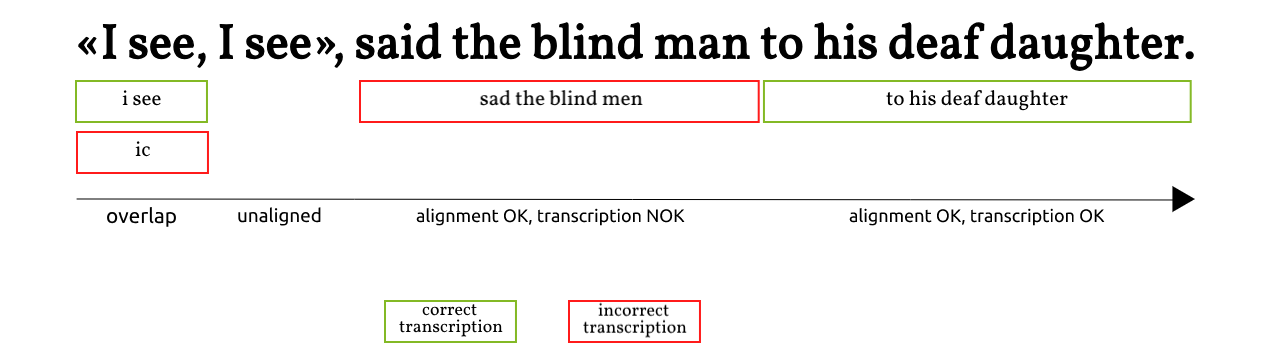
\includegraphics[width=\linewidth]{./img/example_alignment.png}
	\caption{Example for a partially correct alignment of parts of a sentence}
	\label{example_alignment}
\end{figure}

\subsection{Test and results}

The pipeline was evaluated using the model with the lowest average validation-\ac{LER}. For English, this was the model with dropouts. To prevent overfitting, training was stopped after x epochs (early stopping). The pre-trained \ac{DS} model was used as a reference model for comparison.

$P$, $R$ and $F$ were calculated for English and German by running each sample from the test set of the respective corpus through the pipeline.

\subsection{Pipeline performance using an \ac{ASR} model for a different language}

Due to an implementation error the samples from the German test set were run through the pipeline using an \ac{ASR} for English at some point in the testing phase. The error was corrected, but surprisingly enough, the transcripts produced were still accurate enough for alignment. Apparently, the Needle-Wunsch algorithm used in the global alignment stage only needs very little resemblance of the partial transcripts to the real transcripts in order produce alignments that are usable, although maybe a bit worse.
\newpage

\section{Forced Alignment for other languages}

So far, only audio and transcripts in English were considered. A fully automated solution however should be able to align text and audio in any other language. Because of linguistic characteristics like sound patterns and morphology the results might vary a lot between languages when tested underwise identical circumstances. To get some intuition about the influence of language and whether above conclusions are transferable to other languages, the pipeline was evaluated on the German samples received from \textit{ReadyLingua}.

\subsection{Inferring German transcripts}

Enabling the pipeline to handle German samples means training a German \ac{ASR} as its core element. This required minimal modifications to the network architecture, because German transcripts use a different alphabet. As mentioned before, the apostrophe is far less common in German than in English and was therefore dropped. On the other hand, umlauts are very common in German and were added to the 26 ASCII characters. Since the alphabet represents all possible labels, the output layer consisted of 31 units (one for each character in the alphabet, the three umlauts, space plus a blank token) instead of the 29 units used for English.

Training an \ac{ASR} model for German and plotting a learning curve also required amounts of training data on a similar scale like the \ac{CV} corpus used for English. Since at the time of this writing, the \ac{CV} was still a work in progress, datasets for languages other than English were not available. High-Quality \ac{ASR} corpora are generally hard to find, especially considering the number of samples needed to train a \ac{RNN}. There are corpora for \ac{ASR} in German, but those are either not freely available or their quality is unknown. An extensive list of German corpora for various purposes can be found at the \ac{BAS}\footnote{\url{https://www.phonetik.uni-muenchen.de/Bas/BasKorporaeng.html}}. Some of the corpora on this list are free for scientific usage. However, not all of these corpora are targeted at \ac{ASR} and their quality is often unknown.

\subsection{Data augmentation}

Integrating new raw data means preprocessing the audio (e.g. resampling) and the text (e.g. normalization, tokenization) to make sure it exhibits the same properties as the other corpora and the data conforms to the expected format. This step is usually very time consuming, often using up most of the project time. Because no ASR corpus for German was readily available, training was done on the data received from \textit{ReadyLingua} as a start and see how far we get. The alignment between audio and transcript in this corpus was done manually and is therefore very accurate. Audio and text were already preprocessed in the IP8 project and the metadata was processed and stored as a corpus. The individual training samples could therefore be transformed to the expected format with comparably little effort. Also, the samples exhibited similar properties (average audio and transcript length) like the \ac{CV} corpus (refer to table \ref{corpora_stats}). However, the total length of the samples in the training set was only about one and a half hours, which was much less than the 1000+ minutes of the \ac{CV} corpus and certainly not enough for the 1.000 minutes needed to plot a learning curve like to the one made for English. 

An easy way to get more training data is augmenting existing data by synthesizing new data from it. This is particularly easy for audio data, which can be distorted in order to get new samples corresponding to the same transcript. The following distortions were applied in isolation to each sample in the training set:

\begin{itemize}
	\item \textbf{Shifting}: The frames in the input signal were zero-padded with samples corresponding to a random value between $0.5$ and $1.5$ seconds, shifting the signal to the right, i.e. starting the signal later. This resulted in one additional synthesized sample for each original sample. Shifting to the left was not done to prevent cropping parts of the speech signal.
	\item \textbf{Echo}: The presence of echo can be generated with the Pysndfx library\footnote{\url{https://github.com/carlthome/python-audio-effects}} using random values for delay and damping. This resulted in one additional sample.
	\item \textbf{Pitch}: The pitch of the signal was increased or decreased. Increasing and decreasing was done using two different random factors, resulting in two additional samples. This can be seen as a rudimentary way to simulate a female from a male speaker or vice versa.
	\item \textbf{Speed}: Faster or slower speaking rates can be simulated by "stretching" or "compressing" the signal while preserving the pitch. Similar to the change in pitch, two different random factors were use to change the tempo. This resulted in two additional samples.
	\item \textbf{Volume}: The loudness of the speaker was artificially reduced or increased by a random value within the range of $[-15..-5]$ resp. $[5..15]$ db. This resulted in two additional sample.
\end{itemize}

With above methods eight synthetisized samples can be created for each original sample from the corpus. It turned out however that this was still not enough to plot a learning curve. To augment the data to the 1.000 minutes needed, additional samples were created using a random combination of the distortions. The random parameters differed from the ones used before to prevent overfitting to the distortion. Table \ref{corpus_synth_stats} shows the corpus statistics before and after data augmentation.

\begin{table}[!htbp]
	\centering
	\begin{tabular}{|l|r|r|r|r|}
		\hline
		\thead{} & \thead{total audio length} & \thead{\# samples} & \thead{Ø sample length (seconds)} \\
		\hline
		before augmentation & $1:36:09$ & $1,700$ & $2.89$ \\ 		
		after augmentation & $16:40:00$ & $18,955$ & $3.16$ \\ 		
		\hline
	\end{tabular}
	\caption{Comparison of \ac{RL} corpus before and after data augmentation (training set only)}
	\label{corpus_synth_stats}
\end{table}


\subsection{Creating a Language Model for German}

Since the \ac{ASR} stage in the pipeline uses a spell-checker querying a \ac{LM} to post-process the results a $5$-gram model similar to the one created by Mozilla needed to be trained first.

\subsection{n-Gram Language Models}

To understand the following sections better it might be helpful to get a quick recap about \ac{LM}. \ac{LM} are probabilistic models that model the likelihood of a given sequence of characters or words. The most widely used type for word-based models \ac{LM}s are $n$-gram \ac{LM}. However, such models can estimate probabilities only for words that appear in the vocabulary of the corpus they were trained on. All other words are \ac{OOV} words with a probability of $0$. The probability of a sentence can be computed from the probabilities of each word ($1$-grams) with given all its preceding words in the sentence using conditional probability. Getting statistically relevant high numbers for each combination of words requires huge text corpora. However, language is dynamic and new sentences can be created all the time so that no corpus would be big enough. To handle this, $n$-grams approximate the probability of a combination of words by only considering the history of the last $n$ words ($n$ denoting the order). However, above problem is still valid for $n$-grams of any order: Because of combinatorial explosion $n$-grams suffer from sparsity with increasing order. 

\subsubsection{Perplexity, discount and smoothing}

To evaluate an $n$-gram \ac{LM} a metric called \textit{perplexity} is usually used, which is the normalized inverse probability on a test set. The perplexity can be interpreted as the grade to which the \ac{LM} is "confused" by a certain $n$-gram. A high perplexity therefore corresponds to a low probability. Since the perplexity carries the probability of a certain $n$-gram in the denominator, the perplexity for \ac{OOV}-$n$-grams cannot be calculated (division by zero). To handle this efficiently, a technique called \textit{smoothing} is applied. A very rudimentary form of smoothing is \textit{Laplace Smoothing}, which assigns a minimal count of $1$ to every $n$-gram. All other counts are also increased by adding $1$. This prevents counts of zero for $n$-grams that do not appear in the training corpus. Smoothing therefore shaves off a bit of the probability mass from the known $n$-grams and moves it to the unknown $n$-grams. The factor with which the probability of a known $n$-gram is reduced is called \textit{discount}. 

\subsubsection{Kneser-Ney Smoothing}

Although with Laplace Smoothing a very low probability is assigned to previously unseen $n$-grams (which results in a high perplexity), it performs poorly in application because it discounts frequent $n$-grams too much (i.e. gives too much probability to unknown $n$-grams). A better way of smoothing is achieved using \textit{Kneser-Ney Smoothing}. For unseen $n$-grams, \textit{Kneser-Ney Smoothing} estimates the probability of a particular word $w$ being the continuation of a context based on the number of context it has appeared in the training corpus. For any previously unseen $n$-gram, a word that appears in only few contexts (e.g. the word \textit{Kong}, which only follows the words \textit{King} or \textit{Hong} in most corpora) will yield a lower probability than a word that has appeared in many contexts, even if the word itself may be very frequent. The intuition behind this is that such a word is assumed less likely to be the novel continuation for any new $n$-gram than a word that has already proved to be the continuation of many $n$-grams.

\subsection{Creating a raw text corpus}

To train a $n$-gram model for German, a raw text corpus of German Wikipedia articles was used as corpus. Like the English $n$-gram from Mozilla KenLM \parencite{kenlm} was used to estimate the probabilities. The articles were pre-processed to meet the requirements of \textit{KenLM}. It was normalized as follows 

\begin{itemize}
	\item remove Wiki markup
	\item remove punctuation
	\item make everything lowercase
	\item \textbf{Unidecoding}: translate accentuated characters (like \code{è,é,ê}, etc.) and special characters (like the German \textit{ß}) to their most similar ASCII-equivalent (\code{e} resp. \code{ss}). This process helps accounting for ambiguous spelling variants of the same word and misspelled words. It also reduces the number of unique words by reducing different versions to a normalized variant. A special case are umlauts. Although also not part of the ASCII code set, they were kept as-is because they are very common in German.
	\item \textbf{Tokenization}: Because \textit{KenLM} expects the input as sentences (one sentence per line), the raw text was further tokenized into sentences and words using NLTK \parencite{nltk}. 
	\item \textbf{Numeric tokens}: Word tokens that are purely numeric (such as year numbers) are replaced with the special token \code{<num>}. Although such tokens occur frequently in the Wikipedia articles, they are unwanted in the corpus because they represent values and do not carry any semantic meaning. Because there is a infinite number of possible numeric tokens, they were all collapsed to the same normalized token.
\end{itemize}

The corpus was saved as text file containing one normalized sentence per line. The special tokens \code{<s>} and \code{</s>} are used to mark beginnings and endings of sentences as well as the \code{<unk>} token which is traditionally used to represent \ac{OOV} words. They are however not part of the corpus because they are added automatically by \textit{KenLM}.

The following lines are an excerpt of a article in the German Wikipedia along with its representation in the corpus.

\begin{displayquote}[German Wikipedia article about Speech Recognition\footnote{\url{https://de.wikipedia.org/wiki/Spracherkennung}}]
	Die Größe des Wörterbuchs hängt stark von der Sprache ab. Zum einen haben durchschnittliche deutschsprachige Sprecher mit circa 4000 Wörtern einen deutlich größeren Wortschatz als englischsprachige mit rund 800 Wörtern. Außerdem ergeben sich durch die Flexion in der deutschen Sprache in etwa zehnmal so viele Wortformen, wie in der englischen Sprache, wo nur viermal so viele Wortformen entstehen.
\end{displayquote}

\begin{lstlisting}[numbers=left, caption=Representation in corpus]
die grösse des wörterbuchs hängt stark von der sprache ab
zum einen haben durchschnittliche deutschsprachige sprecher mit circa <num> wörtern einen deutlich grösseren wortschatz als englischsprachige mit rund <num> wörtern
ausserdem ergeben sich durch die flexion in der deutschen sprache in etwa zehnmal so viele wortformen wie in der englischen sprache wo nur viermal so viele wortformen entstehen
\end{lstlisting}

Like for the English spell checker, three vocabularies containing the $40.000$, $80.000$ and $120.000$ most frequent words from the corpus was created. The words from these vocabularies make up $87.75\%$, $90.86\%$ resp. $93.36\%$ of the total number of words in the corpus. It is expected that the optimal number of words in the vocabulary is higher for German than for English. This is due to the fact that different flexions of the same word are very common in German due to grammatical conjugations (different forms for the same verb) and declinations (different cases for the same noun). Therefore German tends to apply a wider range of words and the size of vocabulary had to be increased. Handling the different flexions would require lemmatization and/or stemming the corpus in order to reduce them to a common base form. This has not been done for simplicity and time constraints. It is also doubtful whether this would actually help improving the quality of inferred transcripts, since humans do not speak in lemmata or stems.

\subsection{Training the \ac{LM}}

The final corpus contained data from 2,221,101 Wikipedia articles (42,229,452 sentences, 712,167,726 words, 8,341,157 unique words). This corpus was used to train a $5$-gram \ac{LM} using \textit{KenLM}. \textit{KenLM} uses \textit{Kneser-Ney Smoothing} and some optimization techniques called \textit{quantization} and \textit{pointer compression}. 

\subsubsection{Data structures}
$n$-grams can be represented with a prefix-tree structure (called \textit{Trie}) \footnote{note that \textit{KenLM} offers a so called \textit{PROBING} data structure, which is fundamentally a hash table combined with interpolation search, a more sophisticated variant of binary search, which allows for constant space complexity and linear time complexity. This does however not change the fact that $n$-grams can conceptually be thought as a tree of grams}, which allows for pruning. $n$-grams of order 2 and higher can be pruned by setting a threshold value for each order. $n$-grams whose frequency is below the threshold will be discarded. \textit{KenLM} does not support unigram pruning.

\subsubsection{Quantization}
To save memory, the amount of bits used to store the non-negative log-probabilities can be reduced with the parameter $q$ to as little as $q = 2$ bits at the expense of accuracy. This reduction yields $2^q -1$ possible bins. The value of each bin is calculated by equally distributing the probabilities over these bins and computing the average. Note that the quantization is done separately for each order and unigram probabilities are not quantized.

\subsubsection{Pointer Compression}
To use memory even more efficiently, the pointers which are used to store $n$-grams and their probabilities can be compressed. Such pointers are used to represent e.g. word IDs (for $q$-grams) and are stored as sorted integer-arrays. Additionally, These integers can be compressed using a lossless technique from \cite{raj_lossless} by removing leading bits from the pointers and store them implicitly into a table of offsets. The parameter $a$ controls the maximum number of bits to remove. There is a time-space trade-off meaning that a higher value of $a$ will lead to a smaller memory footprint at the cost of a slower training time.

\subsubsection{Building the model}

The a $5$-gram \ac{LM} was trained on the German Wikipedia corpus using  using the Trie data structure and the same parameters like the model downloaded from \textit{DeepSpeech} ($q=8$ and $a=255$). Like the \textit{DeepSpeech} model $4$- and $5$-grams were pruned by setting a minimum frequency of $1$.

%Pruning 1-grams would help getting rid of obvious spelling mistakes and very rare tokens that only appear in very special contexts. Unfortunately, \textit{KenLM} does not support pruning unigrams, only higher-order $n$-grams. Therefore the vocabulary used for training was limited to the 500,000 most frequent words not containing numbers with a minimum length of 2 characters \footnote{this constraint was imposed because NLTK did sometimes not tokenize abbreviations like \textit{z.B.} correctly, which resulting in two separate tokens \code{z} and \code{b}}. Note that this amount is about the same what was used in the \textit{DeepSpeech} paper \parencite{deepspeech} but more than the $250.000$ words used for the English spell checker. 

%The 500k most frequent words in the vocabulary make up 96.42\% of the whole corpus. The most frequent word in the vocabulary is the \code{<num>} token (29,659,021 counts). The least frequent word is \textit{Flachmeeres} (31 counts), which is actually a derivate of another German word \textit{Flachmeer}, which also appears in the vocabulary (109 counts) and which is an example of above mentioned flexion. 

%By limiting the vocabulary to the 500k most frequent words, the unigrams in the KenLM were artificially pruned. The number of unigrams was therefore 500,003 (one unigram for each word in the vocabulary plus one each for the \code{<s>}, \code{</s>} and \code{<unk>} tokens). The $n$-grams used to train the \ac{LM} have been pruned by setting the minimal threshold for $n$-Grams of any order ($n \in 1..4$) to 40. This is the value that Google used (reference from Jurafsky). Pruning unigrams helped getting rid of obvious spelling mistakes and very rare tokens that only appear in very special contexts (like the tokens \textit{aaaaa} or \textit{zzyzzyxx}) (EDIT: Pruning unigrams is not supported by KenLM, but the vocabulary can be limited). Such words are mostly not no real German words and should therefore not be trained on. Pruning higher-order $n$-grams was done to increase performance (both in space and time).

\subsection{Evaluating the \ac{LM}}

Literature suggests two methods to evaluate a \ac{LM}: Extrinsic and intrinsic evaluation.

\subsubsection{Extrinsic and intrinsic evaluation}

The best way to evaluate a \ac{LM}is to embed it in an application and measure how much the application improves \parencite{slp3}. This is called \textit{extrinsic evaluation} and has been done by comparing the learning curves with and without using a \ac{LM}. However, to measure the performance of a \ac{LM} independently (\textit{intrinsic evaluation}) one would have to provide a test set containing unseen sentences an assess the scores of the \ac{LM} on their $n$-grams. The results can then be compared to a reference \ac{LM}: Whatever model produces higher probabilities (or lower perplexity) to the $n$-grams in the test set is deemed to perform better. However, models can only be compared if they use the same vocabulary and always encode characteristics of the training corpus \parencite{slp3}. Since the sentences in a corpus of legal documents use different structures and word distributions than a corpus of children's books, two models trained on these corpora will not be comparable. Evaluating the created German Wikipedia corpus intrinsically would therefore require training a reference model on the same corpus, which can become very time consuming.

\subsubsection{Evaluation of KenLM}

\textit{KenLM} has been extensively compared to other \ac{LM} implementations like \ac{SRILM} both in terms of speed and accuracy. It has been found to be both faster and more memory efficient \parencite{kenlm} than the fastest alternative. Its low memory profile makes it runnable on a single machine, while other algorithms like \textit{MapReduce} target clusters \parencite{kenlm_estimation}. The highly optimized performance was a big advantage especially for this project because it enabled testing the model on a local machine. The probabilistic performance of \textit{KenLM} has been evaluated by training a $5$-gram model on a 126 billion token corpus (393 million unique words) \parencite{kenlm_estimation}. This model was embedded in some Machine Translation systems (Czech-English, French-English and Spanish-English) . Evaluation was done by calculating the BLEU score and comparing it to embeddings of other \ac{LM}. \textit{KenLM} placed first in all submissions.

\subsubsection{Evaluation of the German Wikipedia \ac{LM}}

Because of time constraints and because \textit{KenLM} has already been extensively evaluated on English I resigned from evaluating my German \ac{LM} intrinsically, even though the corpus used for training is not as big as the one used in \cite{kenlm_estimation}. \textit{KenLM} is to date widely recognized as the best performing \ac{LM} available, which is also emphasized by the usage of a \textit{KenLM} model in the Mozilla implementation of \textit{DeepSpeech}.

To still get an intuition about how well the model performs, two different experiments were made:

\begin{itemize}
	\item \textbf{Experiment 1}: The probability calculated for valid German sentences was compared against variants of the same sentences with the words in randomized order.
	\item \textbf{Experiment 2}: The \ac{LM} was used together with its vocabulary to build a simple word predictor.
\end{itemize}

Both experiments are explained in more depth below.

\subsubsection{Evaluation 1: Comparing scores of randomized sentences}

The first experiment tests the validity of the probabilities (\textit{scores}) calculated by the \ac{LM}. For this, an arbitrary choice of 5 valid sentences in German was used. To ensure the sentences could not have been seen during training, the following 5 sentences were taken from a newspaper printed after the creation of the Wikipedia dump:

\begin{lstlisting}[numbers=left, caption=Representation in corpus]
Seine Pressebeauftragte ist ratlos.
Fünf Minuten später steht er im Eingang des Kulturcafés an der Zürcher Europaallee.
Den Leuten wird bewusst, dass das System des Neoliberalismus nicht länger tragfähig ist.
Doch daneben gibt es die beeindruckende Zahl von 30'000 Bienenarten, die man unter dem Begriff «Wildbienen» zusammenfasst.
Bereits 1964 plante die US-Airline Pan American touristische Weltraumflüge für das Jahr 2000.
\end{lstlisting}

All sentences have been normalized the same way sentences were preprocessed for training. For each of them the score was calculated. Then the words were shuffled and the score was calculated again. A good \ac{LM} should calculate a (much) higher probability for the original sentence, because the shuffled sentence is most likely just gibberish.  Table \ref{LM_evaluation} shows the results of the comparison. It is evident that the probabilities for the shuffled sentences are much lower than for the sentences where the words appear in the correct order. The probabilities calculated by the \ac{LM} are therefore deemed valid.

\begin{table}[!htbp]
	\centering
	\begin{tabular}{|l|r|l|r|}
		\hline
		\thead{original sentence (normalized)} & \thead{score} & \thead{permuation} & \thead{score} \\
		\hline
		\makecell[l]{seine pressebeauftragte\\ist ratlos} & -17.58 & \makecell[l]{ist ratlos\\pressebeauftragte seine} & -21.52 \\
		\hline
		\makecell[l]{fünf minuten später steht\\er im eingang des kulturcafes\\an der zürcher europaallee} & -40.23 & \makecell[l]{des er minuten zürcher kulturcafes\\steht europaallee eingang\\fünf im später an der} & -57.69 \\
		\hline
		\makecell[l]{den leuten wird bewusst\\dass das system des \\ neoliberalismus nicht\\länger tragfähig ist} & -35.52 & \makecell[l]{system nicht das ist\\dass leuten tragfähig des\\neoliberalismus den\\bewusst länger wird} & -51.27 \\
		\hline
		\makecell[l]{doch daneben gibt es die\\beeindruckende zahl von \code{<num>}\\bienenarten die man unter dem\\begriff wildbienen zusammenfasst} & -48.36 & \makecell[l]{dem gibt wildbienen zahl\\beeindruckende doch man\\zusammenfasst es daneben bienenarten\\von die unter die \code{<num>} begriff} & -75.95 \\
		\hline
		\makecell[l]{bereits \code{<num>} plante\\die usairline pan american\\touristische weltraumflüge\\für das jahr \code{<num>}} & -58.04 & \makecell[l]{plante touristische für\\jahr pan american das\\bereits usairline \code{<num>}\\\code{<num>} weltraumflüge die} & -64.02 \\
		\hline
	\end{tabular}
	\caption{Comparison of log10-probabilities calculated for news sentences and a permutation of their words}
	\label{LM_evaluation}
\end{table}

\subsubsection{Experiment 2: Word predictor}

The second experiment tests whether the trained \ac{LM} is able to continue a sentence given its beginning. For this each word from the vocabulary is appended and the score of the resulting stumps is calculated. The most likely continuation can be estimated by sorting the resulting list in descending order (the probabilities are $\log_10$-based, i.e. negative) and taking the first element. This behavior can be applied iteratively to construct a sentence from a stump. For this experiment a sentence was started with the stump \foreignquote*{french}{\textit{Ein 2007 erschienenes}}. Afterwards a word from the five most probable continuations was appended. The extended stump was then again fed into the \ac{LM}. This process was repeated until some kind of sentence ending was encountered. Each extended stump was preprocessed the same way the sentences were preprocessed for training (lowercasing, replacing numbers with \code{<num>}, etc.). Figure \ref{word_predictor} shows the path taken through the predictions. Note that the predictions for the second and third word of the stump after typing the first word are shown in grey for illustrative purposes, although they were not considered for continuation.

\begin{figure}[h!]
	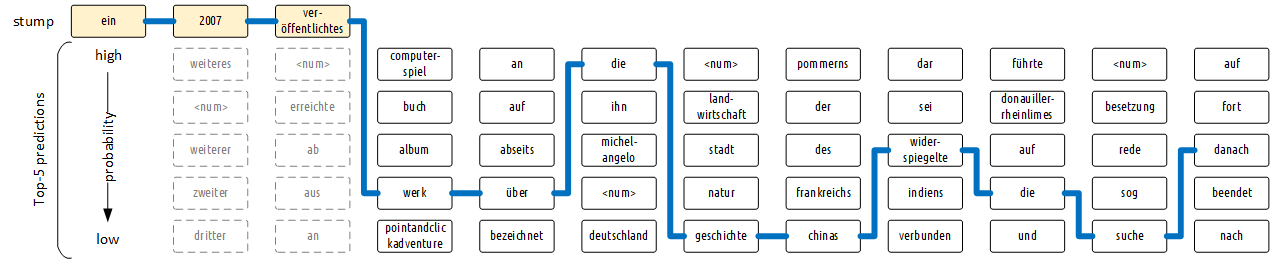
\includegraphics[width=\linewidth]{./img/word_predictor.png}
	\caption{Word predictions of the trained 5-gram model for continuations of the stump \foreignquote*{french}{\textit{Ein 2007 erschienenes ...}}. The blue path represents a grammatically valid German sentence.}
	\label{word_predictor}
\end{figure}

Although prediction was slow we can observe that the words suggested by the \ac{LM} are generally grammatically correct continuations and often make sense, although the probability for some of the predicted words (like \textit{Michelangelo}) is sometimes unexplicably high. Nevertheless it was possible to create a valid German sentence from the stump using only the suggested words. The \ac{LM} even seems to have captured some notion about grammatical concepts like German cases (e.g. that \foreignquote{french}{\textit{die Geschichte Chinas}} is more likely than \foreignquote{french}{\textit{die Geschichte China}}). On the other hand we can observe that the meaningfulness of the suggestions decreases with the progress because some long-distance relationships between words are lost for small values of $n$.

\subsection{Results}

The following figures show the learning curve for training on the German with synthetisation.
\newpage

\section{Conclusion}\label{conclusion}

Was man auch noch machen könnte:

- Zusätzliche Daten/Korpora: Bavarian ARchive for Speech Signals (http://www.bas.uni-muenchen.de/forschung/Bas/BasKorporaeng.html)
- Hunspell Checker: http://hunspell.github.io/
  --> Python modul: https://github.com/blatinier/pyhunspell
  --> Dictionaries gibt's hier https://github.com/wooorm/dictionaries
- Transfer Learning (müsste man aber zuerst ein geeignetes Modell finden) und Layer freezen
 --> Layer freezen
\newpage

\listoffigures
\listoftables

\newpage
\printbibliography

\newpage
\section*{Acronyms used in this document}

\begin{acronym}[Bash]
	\acro{ASR}[ASR]{Automatic Speech Recognition}
	\acro{CTC}[CTC]{Connectionist Temporal Classification}
	\acro{DS}{Deep Speech}
	\acro{E2E}{end-to-end}
	\acro{FA}[FA]{Forced Alignment}
	\acro{FHNW}[FHNW]{University of Applied Sciences}
	\acro{GPU}[GPU]{Graphics Processing Unit}
	\acro{GRU}{Gated Recurrent Unit}
	\acro{LER}[LER]{Label Error Rate}
	\acro{LM}[LM]{Language Model}
	\acro{LSTM}{Long Short Term Memory}
	\acro{LSA}[LSA]{Local Sequence Alignment}
	\acro{MFCC}[MFCC]{Mel-Frequency Cepstral Coefficients}
	\acro{NN}{Neural Network}
	\acro{RNN}[RNN]{Recurrent Neural Network}
	\acro{SGD}{Stochastic Gradient Descent}
	\acro{STT}[STT]{Speech-To-Text}
	\acro{OOV}{Out Of Vocabulary}
	\acro{SRILM}{the SRI Language Modelling Toolkit}
	\acro{SW}{Smith Waterman}
	\acro{VAD}[VAD]{Voice Activity Detection}
	\acro{WER}[WER]{Word Error Rate}
\end{acronym}

\newpage
\section{Ehrlichkeitserklärung}
Hiermit erkläre ich, dass ich die vorliegende schriftliche Arbeit
selbstständig und nur unter Zuhilfenahme der in den Verzeichnissen oder
in den Anmerkungen genannten Quellen angefertigt habe. Ich versichere
zudem, diese Arbeit nicht bereits anderweitig als Leistungsnachweis
verwendet zu haben. Eine Überprüfung der Arbeit auf Plagiate unter
Einsatz entsprechender Software darf vorgenommen werden.\\
Würenlingen, \today\\[4\baselineskip]
Daniel Tiefenauer
\end{document}